\subsection{Deep Learning}\label{sec:deep-learning}

As previously mentioned, the growth of \acf{DL} began in the early 2000s as a response to the challenge of handling vast quantities of data. Fundamentally, \ac{DL} stems from the application of \ac{ML} to process large amounts of data. To be precise, \ac{DL} is a subfield of \ac{ML} that employs multiple levels of information processing and abstraction to learn and represent features, as demonstrated by Deng et al. \cite{deng_deep_2014}. Subsequently, the extracted features can be utilized for classification, regression, and other modeling techniques. In the past, such features were manually selected by humans.

This study uses \ac{DL} for sound generation because it offers several advantages over traditional sound generation techniques. By being data-driven, these models can generate new sounds based on sounds it has heard before. On traditional methods, these sounds would have to come from the inspiration of their human creator. Besides, end-to-end generation, from text to sound generation, is only possible through \ac{DL}. The model has to extract features from the text, learn features from thousands or millions of sounds, and correlate both. This highly complex task can only be achieved with \ac{DL} techniques.

This section presents traditional \ac{DL} architectures and their evolution to generative \ac{DL} architectures.

%%%%%%%%%%%%%%%%%%%%%%%%%%%%%%%%%%%%%%%%%%%

\subsubsection{Deep Learning Architectures}

Generative \ac{DL} architectures establish blueprints for developing \ac{DL} networks that synthesize diverse and novel data samples according to a learned distribution. These architectures entail creating latent data constructs and learning to emulate the fundamental statistical patterns found in observed data.

Generative deep neural models have been applied to tasks comprising image synthesis, text generation, and audio synthesis. Their popularity has recently surged owing to their remarkable ability to generate high-quality data and effectively model complex distributions. In the following sections, we outline the most ordinarily used generative \ac{DL} architectures, presented chronologically, as summarized in Table~\ref{tab:archs}.

\begin{table*}[ht]
\centering
\caption{Comparison of Generative Deep Learning Architectures}
\label{tab:archs}
\begin{tabularx}{\textwidth}{|p{20mm}|c|p{25mm}|X|c|}
\hline
\textbf{Model} & \textbf{Year} & \textbf{Type} & \textbf{Key Characteristics} & \textbf{Inference} \\ \hline
DARN & 2013 & Autoregressive & Uses a single model to predict the probability distribution of each output token conditioned on the previous tokens & Sequential \\ \hline
VAE & 2013 & Variational Autoencoder & Learns a latent representation of the input data and generates new samples by sampling from the learned latent space & Parallel \\ \hline
GAN & 2014 & Generative Adversarial Network & Consists of a generator and a discriminator that compete in a two-player minimax game to generate realistic samples & Parallel \\ \hline
Normalizing Flows & 2015 & Flow-based models & Transforms a simple probability distribution into a complex one by applying a sequence of invertible transformations & Parallel \\ \hline
Diffusion & 2015 & Flow-based models & Uses a diffusion process to model the probability distribution of the data & Parallel \\ \hline
Transformers & 2017 & Attention-based models & Uses self-attention to capture global dependencies and generate sequences & Sequential \\ \hline

VQ-VAE &
    2018 &
    Variational Autoencoder &
    Discretizes the continuous latent space by mapping each latent vector to the closest codebook vector &
    Parallel \\ \hline

MS-VQ-VAE &
    2019 &
    Variational Autoencoder &
    Is an extension of the VQ-VAE that incorporates multiple discrete latent spaces of different scales, enabling hierarchical and diverse representations with improved abstraction levels and latent space expressiveness &
    Parallel \\ \hline

\end{tabularx}
\end{table*}

This section will discuss novel architectural designs for \ac{DL}. It is important to note that there is a discrepancy between the date of their conceptualization and their widespread adoption. This trend is common in machine learning because software theories have a faster rate of development compared to hardware theories.

This section does not describe all \ac{DL} architectures that had some relevance. It, however, describes the ones used either by the models developed or by systems studied for the state-of-the-art.

\paragraph{Feedforward Neural Network (1957)} \label{sec:feedforward}

To understand \textit{feedforward neural networks} (or any neural network), it is essential to understand both Hebbian learning and the perceptron.

In 1949, inspired by the observation that neurons that fire together wire together, the psychologist Donald Hebb \cite{hebb_organization_1949} developed a rule for adjusting the strength of connections between neurons in any neural network. The rule goes by the name of Hebbian learning and states that if two neurons are activated simultaneously, their connection should be strengthened. The idea behind Hebbian learning is that learning occurs as a result of changes in the strengths of synaptic connections between neurons in the brain rather than solely due to changes in the activity of individual neurons.

The perceptron is a simple model first published in 1958 by F. Rosenblatt \cite{rosenblatt_perceptron_1958}. It consists of a single neuron with a binary threshold --- also known as bias --- and is used for binary classification tasks. A set of weights transforms the input to the perceptron. The output is determined by checking if the input is enough to trigger the bias and then applying a function to the weighted sum of inputs as shown in Figure \ref{fig:perceptron}. The output of the perceptron can be mathematically expressed as in the equation \ref{eq:perceptron-ouput}.

\begin{equation} \label{eq:perceptron-ouput}
    y = h(\sum_{x=1}^N (I_x \times W_x) - b)
\end{equation}

$y$ is the output, $N$ is the number of inputs, $I_n$ is the input number $n$, $W_n$ is the weight related to $I_n$, $b$ is the bias, and $h$ is an activation function, usually.

The perceptron is trained using an algorithm that adjusts the weights based on the error between the actual and predicted outputs. The exciting part is that Hebbian learning can be applied to perceptrons, which was one of the bases of the future backpropagation. The perceptron can only classify linear separated sets, as shown in \textit{Perceptrons} \cite{marvin_minsky_perceptrons_1969}, hence the need for more complex structures.

\begin{figure}[ht]
    \centering
    \ctikzfig{figures/2-sota/perceptron}
    \caption[Perceptron]{\textbf{Perceptron} --- The perceptron receives multiple inputs associated with a weight. It also holds a given bias. Its output is the application of a given function (\textit{e.g.} step function) to the weighted average of the inputs minus the bias.}
    \label{fig:perceptron}
\end{figure}

A feedforward neural network is no more than a set of layers of perceptron-like neurons. In a feedforward neural network, information moves in only one direction --- forward. Hebbian learning no longer applies to these networks, so more complex algorithms, such as backpropagation, are required. These networks are universal approximators \cite{cybenko_approximation_1989} if they have at least one hidden layer, meaning they can approach any function given the proper configuration. They can also learn different tasks than classification, such as regression. The first functional networks, called multi-layer perceptrons, were invented in the 1980s. An example structure of a feedforward neural network can be seen in Figure \ref{fig:feed_forward_neural_network}.

\begin{figure}[!ht]
    \centering
    \ctikzfig{figures/2-sota/feed-forward-neural-network}
    \caption[Feedforward Neural Network]{\textbf{Feedforward neural network} --- The size of the input is constant. The flow of information goes through nonlinear functions on hidden layers. Both weights between nodes on different layers and the nodes' bias are trained with backpropagation.}
    \label{fig:feed_forward_neural_network}
\end{figure}

To a certain extent, since the perceptron is the most basic feedforward neural network (consisting of only one neuron), these networks do not necessarily equate to deep learning (\ac{DL}). Smaller networks have existed and been utilized for decades. Nevertheless, the foundation for most \ac{DL} architectures comes from this, making it essential to recognize.
\paragraph{Convolutional Neural Network (CNN) (1980)} \label{sec:CNN}

During the 1950s and 1960s, Hubel and Wiesel~\cite{hubel_receptive_1959}, who were distinguished neurophysiologists, conducted pioneering research on the eyes of cats. Their research uncovered the presence of neurons with receptive fields that map various visual regions. Receptive fields refer to specific areas in the visual field that activate particular cells. Their studies revealed two fundamental categories of cells involved in visual processing: simple cells with a strong response to edges and complex cells with larger receptive fields that prioritize the organization of edges over their precise positioning.

In 1980, Kinihiko Fukushima introduced the \textit{neocognitron} which marked a significant milestone in the development of \acp{CNN} \cite{fukushima_neocognitron_1980}. It was one of the first \ac{CNN} architectures designed to mimic specific aspects of human visual perception. This laid the groundwork for future advances in deep learning for computer vision tasks.

\Acp{CNN} are a category of \ac{DL} neural networks widely used in computer vision and other sequential data types. The architecture of \acp{CNN} is specifically designed to handle inputs where data correlate with its vicinity.

The key idea behind \acp{CNN} is to learn and extract features from the input hierarchically. This is achieved through convolutional layers, where a small set of learnable filters are used to scan and transform the input image into a feature map. These networks also use pooling layers that perform down-sampling of the feature map to reduce its size while retaining important information. These operations allow the network to capture patterns and features in the input, which can then be passed to feedforward neural networks and used for classification or regression. This process is represented in Figure \ref{fig:cnn}.

\begin{figure}[ht]
    \centering
    \ctikzfig{figures/2-sota/cnn}
    \caption[Convolutional Neural Network]{\textbf{\Acf{CNN}} --- The network present in the Figure deals with 2D data, such as images. The networks' first step consists of convolutional (and pooling) layers. This first step is responsible for finding features. The deeper the convolutional layer, the bigger the receptive field; consequently, the more abstract the feature. After the features are caught, the flatten operation transforms the data into a 1D vector. And then, the network is no more than a feedforward neural network to, in this case, classify what was fed to the network.}
    \label{fig:cnn}
\end{figure}

A major benefit of \acp{CNN} compared to other kinds of networks is their ability for parallelism, where a long input sequence can be handled fast \cite{huzaifah_deep_2021}. This can greatly accelerate training since the whole output can be processed in one forward pass. The shared weights and local connectivity among neurons in the network enable efficient computation, and using pooling layers lowers the number of parameters to be learned.
\paragraph{Convolutional Operations} \label{sec:conv-layers}

This section will discuss three common layers in \acp{CNN}: convolutional layers, pooling layers, and transposed convolutions. It also introduces the concept of masked convolutions and their applications in specific tasks.

\label{sec:conv-layer}

A \textbf{convolutional layer} is a fundamental building block of \acp{CNN} (see Section \ref{sec:CNN}).

At a high level, a convolutional layer applies a set of learnable filters to the input data, extracting local features and patterns relevant to the task. The filters are typically small and slide over the input data, computing the dot product between the filter weights and the input values at each position. This operation is called convolution and can be seen in Figure \ref{fig:conv-layer}.

\begin{figure}[ht]
    \centering
    \ctikzfig{figures/2-sota/conv}
    \caption[Convolutional layer]{\textbf{Convolutional layer} --- The presented diagram depicts a 1-dimensional convolutional layer designed to process an input signal consisting of a single channel and a length of 7. The layer employs a single filter with a size of 3, resulting in an output signal of length 5 and a single channel. Each element of the output signal is produced by convolving the corresponding filter weights with a subset of the input signal. Specifically, the first output element is generated by convolving the filter with the first three elements of the input signal. The filter is then slid along the input signal with a stride of 1, such that each subsequent output element depends on a different subset of the input signal.}
    \label{fig:conv-layer}
\end{figure}

To be more precise, let us consider a 1D convolutional layer that takes an input tensor $X$ of size $C_{in} \times L_{in}$, where $C_{in}$ is the number of input channels and $L_{in}$ is the length of the input sequence. The layer also has $C_{out}$ filters, each of size $C_{in} \times k$, where $k$ is the size of the filter kernel. The output of the layer is a tensor $Y$ of size $C_{out} \times L_{out}$, where $L_{out}$ is the length of the output sequence.

The convolution operation can be expressed as follows:

\begin{equation}
	Y_{c,i} = \sum_{p=0}^{k-1}\sum_{k=0}^{C_{in}-1} X_{k,i+p} \cdot W_{c,k,p} + b_c
\end{equation}

where $c$ is the index of the output channel, $i$ is the spatial index of the output sequence, $p$ is the spatial index of the filter kernel, $k$ is the index of the input channel, $X_{k,i+p}$ is the input value at position $(k,i+p)$, $W_{c,k,p}$ is the weight of the filter at position $(c,k,p)$, and $b_c$ is the bias term for the $c$-th output channel.

The convolution operation is applied independently to each output channel and each spatial location of the output feature map, resulting in a set of feature maps that capture different aspects of the input data. The weights and biases of the filters are learned during training using backpropagation and gradient descent (see section \ref{sec:backpropagation}), optimizing a suitable loss function for the task at hand.

% alskjdaslkjdasld

\label{sec:pooling}

\textbf{Pooling} is a standard operation in \acp{CNN} that reduces the spatial dimensions of the input feature maps while retaining important information. Pooling is typically applied after convolutional layers to gradually reduce the feature maps' spatial dimensions and increase the network's receptive field. There are several types of pooling, including max pooling, average pooling, L2 pooling, and more. Of these, max pooling is one of the most commonly used.

\textbf{Max pooling} works by partitioning the input feature map into non-overlapping rectangular regions, called pooling kernels. For each pooling kernel, the maximum value is selected and used as the output value for that region. The size of the pooling kernel and the stride determine the amount of reduction in the spatial dimensions of the feature map. The stride is the number of pixels that the pooling kernel is shifted horizontally and vertically between each pooling operation. It can be seen in the Figure \ref{fig:pool}

\begin{figure}[ht]
    \centering
    \ctikzfig{figures/2-sota/pool}
    \caption[Pooling layer]{\textbf{Pooling layer} --- The Figure illustrates a $4 \times 4$ input tensor with a single channel. Each colored square in the tensor denotes a single element. The pooling layer partitions the input tensor into non-overlapping $2 \times 2$ regions and applies a pooling function to each region, resulting in a $2 \times 2$ output tensor with a single channel. The number of channels remains unchanged in this scenario, implying that the pooling function is applied separately to each channel of the input tensor, and the resulting output tensor retains the same number of channels as the input tensor. The primary objective of pooling layers is to decrease the spatial dimensions of the input tensor while maintaining the essential features. In this instance, the pooling layer decreases the spatial dimensions of the input tensor by half, resulting in a smaller output tensor. The output tensor is displayed on the right-hand side of the image, where each colored square represents a single element of the output tensor. The colors of the output tensor correspond to those of the input tensor regions from which they were derived.}
    \label{fig:pool}
\end{figure}

Max pooling has several benefits for \acp{CNN}~\cite{riesenhuber_hierarchical_1999}:
\begin{itemize}
    \item It helps to reduce the model's sensitivity to minor variations in the input. This is because the maximum value within each pooling kernel is selected, which is less sensitive to slight variations than taking the average or other statistics.
    \item It can prevent overfitting by reducing the number of parameters in the model. This is because the pooling operation reduces the spatial dimensions of the feature map, reducing the number of parameters in the subsequent layers of the network.
    \item It can increase the network's receptive field by combining the information from neighboring pixels.
\end{itemize}

There are some potential drawbacks to max pooling as well. One is that it can discard some information that may be important for the task. This is because only the maximum value within each pooling kernel is selected, and other information is discarded.

%laskdjl kajsdlkajs ldkja

\label{sec:transpoed-conv}

A \textbf{transposed convolution}, also known as a deconvolution, is a layer that performs the opposite operation of a convolutional layer. It takes an input tensor of size $C_{in} \times L_{in}$ and produces an output tensor of size $C_{out} \times L_{out}$, where $C_{in}$ and $C_{out}$ are the number of input and output channels, respectively, and $L_{in}$ and $L_{out}$ are the input and output lengths.

The transposed convolution applies a set of learnable filters to the input data. However, instead of sliding the filters over the input, it slides them over the output and computes the dot product between the filter weights and the output values at each position. This operation can be seen as an ``unfolding'' of the convolution operation. Hence the name ``transposed convolution''. An example can be seen in Figure \ref{fig:trans-conv}.

\begin{figure}[ht]
    \centering
    \ctikzfig{figures/2-sota/trans-conv}
    \caption[Transpoed convolution]{\textbf{Transposed convolution} --- This illustration shows how a transposed convolution operation works. The input array has three elements $(3, 4, 3)$ and is shown by the dark blue rectangles at the top. The filter array also has three elements $(5, 5, 2)$ and is shown by the green rectangles in the middle. The output array is obtained by sliding the filter over the input array and computing the element-wise products and sums. The stride parameter controls how much the filter moves, which is 1 in this example. The light blue rectangles at the bottom show the intermediate and final output arrays. The intermediate output arrays are $(15, 15, 6, 0, 0)$, $(0, 20, 20, 8, 0)$, and $(0, 0, 15, 15, 6)$. The final output array is the sum of the intermediate output arrays $(15, 35, 41, 23, 6)$. The gray-shaded regions indicate how the filter broadcasts each element in the input array to produce an intermediate output array.}
    \label{fig:trans-conv}
\end{figure}

The transposed convolution can be expressed as follows:

\begin{equation}
	X_{k,i} = \sum_{p=0}^{k-1}\sum_{c=0}^{C_{out}-1} Y_{c,i+p} \cdot W_{c,k,p} + b_k
\end{equation}

where $k$ is the index of the input channel, $i$ is the spatial index of the input sequence, $p$ is the spatial index of the filter kernel, $c$ is the index of the output channel, $Y_{c,i+p}$ is the output value at position $(c,i+p)$, $W_{c,k,p}$ is the weight of the filter at position $(c,k,p)$, and $b_k$ is the bias term for the $k$-th input channel.

Like convolutional layers, the weights and biases of the filters are learned during training using backpropagation and gradient descent.

\label{sec:masked-conv}

A \textbf{masked convolution} is a convolutional layer that selectively masks out specific input values based on their position in the input sequence. This masking is typically done by setting the weights of the filters to zero for certain positions in the kernel. For example, in an \ac{AR} language modeling task, where the goal is to predict the next word in a sentence given the previous words, a masked convolution can ensure that the model only has access to the previous, not the future words.

Another example where masked convolutions can be helpful is in audio generation tasks. In such tasks, the model takes as input a sequence of audio samples and generates a new sequence of samples that sound similar to the input. In some cases, generating audio that only depends on the previous time steps rather than the entire input sequence may be desirable. This can be achieved using a masked convolution that masks out the future time steps by setting the filter weights to zero for those positions in the kernel. By doing so, the model can only rely on the previous time steps to generate the following sample.

Masked convolutions can be implemented using standard convolutional layers with appropriate masking of the filter weights. Another approach is using a specialized masked convolutional layer that takes an additional mask tensor as input, indicating which input values should be masked.

One advantage of masked convolutions is that they can help prevent the model from overfitting to the training data by forcing it to rely on the input data available at each time step rather than the ground truth values that may not be available at test time. This can be particularly useful in tasks where the input data has a sequential or temporal structure, and the model needs to make predictions based on partial information.

\paragraph{Recurrent Neural Network (RNN) (1986)} \label{sec:rnn}

In 1986, Rumelhart and McClelland, psychologists, in the aftermath of the discovery of the backpropagation algorithm, wrote a book \cite{rumelhart_parallel_1986} where, between others, they took the declarations made in Perceptrons \cite{marvin_minsky_perceptrons_1969}, presented in Section \ref{sec:context}, and showed that, although the perceptron alone might not be enough, networks of perceptrons, with the suitable algorithms, might suffice.

One example they gave was a theoretical network that would be recursive \cite{rumelhart_learning_1987}. This would be the first time the ``recurrent'' term would appear in the literature. They explained that a recursive network is a feedforward network where some weights are kept the same between layers. They showed that it is easy to backpropagate the error and train such a network with this simplification. At the time, ``the major problem with this procedure is the memory required''. This new network was able to solve problems related to sequences. In this chapter, they showed the development of a system that would learn to complete straightforward sentences using \aclp{RNN}.

Furthermore, a \ac{RNN} used nowadays is not very different from the one theorized in 1986. A \ac{RNN} is a neural network derived from a feedforward neural network (see Section~\ref{sec:feedforward}), where some connections between nodes can create cycles. This is because some nodes' output is the same nodes' input. This operation makes the network have memory. These networks can exhibit temporal behavior and process variable-length sequence of inputs. In 1996 it was shown that \acp{RNN} could perform any operation that a regular computer can, meaning that they are Turing complete \cite{hyotyniemi_turing_1996}.

\Ac{RNN} have the problem of forgetting terms seen long ago as new terms come along~\cite{hochreiter_long_1997}. This may be a problem in, for instance, long texts where the model has to remember the name of a given entity that was given at the beginning of the text.

Learning happens as in feedforward neural networks with one additional step: the recurrent nodes are unrolled, as seen in Figure \ref{fig:rnn}.

\begin{figure}[!ht]
    \centering
    \ctikzfig{figures/2-sota/rnn}
    \caption[Simple recurrent neural network]{\textbf{Simple \acl{RNN}} --- The left side of the image displays the most straightforward representation of a \ac{RNN} because it only has one recurrent neuron. Apart from the bias, the neuron has an input weight, a weight for the recursive connection, and a weight for the output. The images on the left and the right are equivalent. The image on the right represents the same simple network. However, it shows what exactly happens when it receives multiple inputs: an output is generated for each one, and a value is passed to the next iteration. One may notice that even though the inputs and outputs change, the weights on the edges do not.}
    \label{fig:rnn}
\end{figure}

New takes that solve the problems with \acp{RNN} have been developed over the years. The basis of these models is to include learnable gates that choose what and when to remember and to forget. The most prominent examples are the \Acfp{GRU} \cite{cho_properties_2014}, and the \Acfp{LSTM} \cite{hochreiter_long_1997}.
\paragraph{RNN Variants} \label{sec:rnn-variants}

\Acp{RNN} are a class of neural networks designed to handle sequential data. They work by maintaining an internal state or memory, which allows them to process sequences of inputs and produce outputs that depend on previous inputs. This definition allows for other types of networks, different from the one shown in the previous section.

However, there are convincing reasons to investigate architectures beyond the basic approach. The typical \ac{RNN} is not without its difficulties, particularly the development of the \textit{vanishing gradient problem} as a major concern.

\Acp{RNN} may be prone to the vanishing gradient problem due to their method of updating internal states. \Acp{RNN} compute the internal state at time step $t$ by incorporating the input of time step $t$ and the previous state of time step $t-1$. This process generates a sequence of dependencies between the present and past states, which leads to multiple matrix multiplications during the backpropagation.

As the gradient keeps decreasing after each multiplication, it may ultimately shrink to such an extent that the neural network fails to learn long-term patterns present in the input sequence.

The prime example of an architecture that fights the vanishing gradient problem is the \textbf{\acf{LSTM}} \cite{hochreiter_long_1997}. \Acp{LSTM} were introduced in 1997 and have since become a popular choice for processing sequential data, especially in \ac{NLP}.

The main idea behind \ac{LSTM} is to introduce memory cells that can selectively forget or remember information from previous time steps. Each memory cell has three gates: the input gate, the forget gate, and the output gate, which control the flow of information into and out of the cell. One can see how these work in Figure \ref{fig:lstm}.

\begin{figure}[ht]
    \centering
    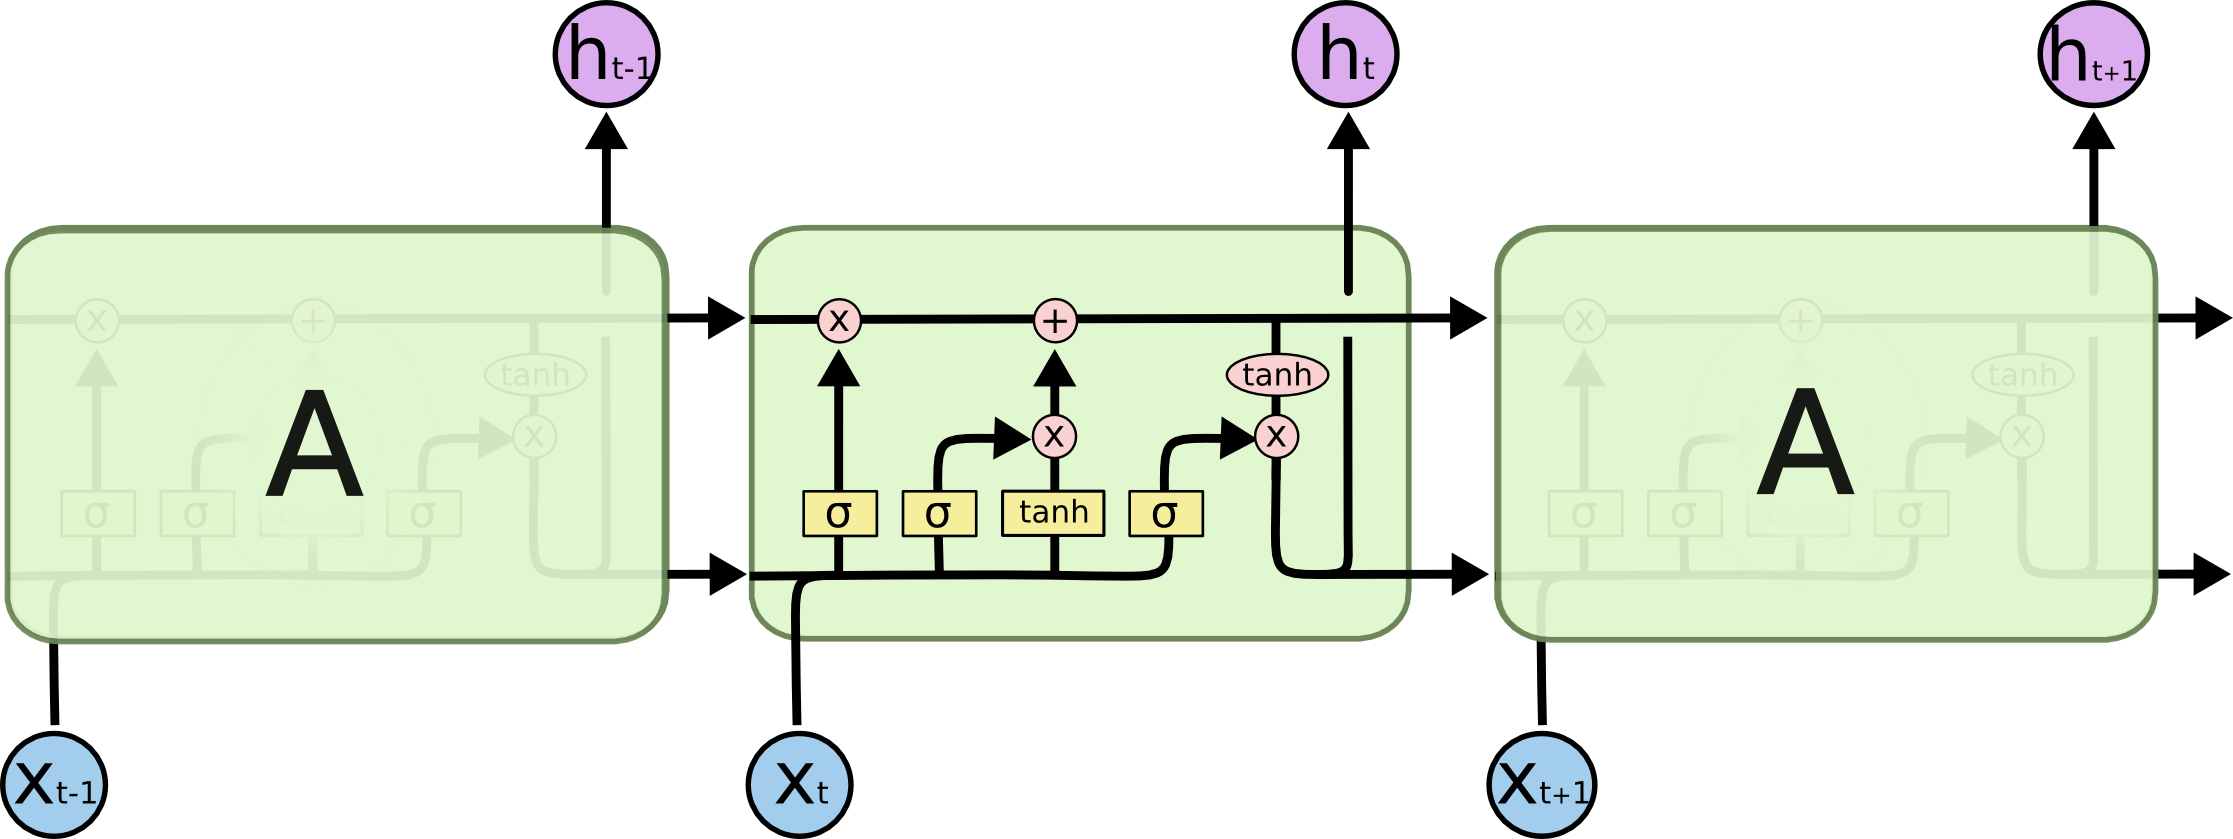
\includegraphics[width=\textwidth]{figures/2-sota/LSTM3-chain.png}
    \caption[Long Short-Term Memory]{\textbf{\Acf{LSTM}} --- 
    The network was taken from \cite{christopher_olah_understanding_2015}. Each green rectangle is an \ac{LSTM} cell. The blue circles represent an input at a given time, such that $X_t$ is the input at time $t$. The pink circles represent the output at a given time $h_t$. Each \ac{LSTM} cell takes three inputs: the previous cell`s memory and output, and the current input, and outputs both the real output and the current memory. In the Figure, the top exiting arrow corresponds to the memory, while the bottom corresponds to the output. The yellow rectangles have learnable parameters, weights, and biases.}
    \label{fig:lstm}
\end{figure}

The forget gate determines which information from the previous state should be forgotten or retained. It takes the current input, $X_t$, and the previous state, $H_{t-1}$, and computes the gate activation, $f_t$, a number between 0 and 1 that determines how much of the previous state should be retained or forgotten. It is calculated as

\begin{equation}
    f_t = \sigma (W_f * [H_{t-1}, X_t] + b_f)    
\end{equation}

$W_f$ is the weight matrix for the forget gate, and $b_f$ is the bias vector.

The input gate determines which information from the current input and the previous state should be allowed into the cell. It takes the current input, $X_t$, and the previous state, $H_{t-1}$, as inputs and computes the gate activation, $i_t$, which is a number between 0 and 1 that determines how much of the input and previous state should be allowed into the cell. It is calculated as

\begin{equation}
    i_t = \sigma (W_i * [H_{t-1}, X_t] + b_i)
\end{equation}

where $\sigma$ is the sigmoid activation function, $W_i$ is the weight matrix for the input gate, and $b_i$ is the bias vector.

The memory update computes the new information stored in the memory cell. It takes the current input, $X_t$, and the previous state, $H_{t-1}$, as inputs and computes the new candidate memory content, $\tilde{C_t}$. It is calculated as

\begin{equation}
    \tilde{C_t} = \tanh (W_C \times [H_{t-1}, X_t] + b_C)
\end{equation}

$W_C$ is the weight matrix for the candidate memory update, and $b_C$ is the bias vector.

The memory cell stores the current memory content, $C_t$, a combination of the previous and new candidate memory content, as determined by the input and forget gates. It is calculated as

\begin{equation}
    C_t = f_t \times C_{t-1} + i_t * \tilde{C_t}
\end{equation}

The output gate determines which information from the current memory cell should be used as output. It takes the current input, $X_t$, and the previous state, $H_{t-1}$, as inputs and computes the gate activation, $o_t$, a number between 0 and 1 that determines how much of the memory cell content should be outputted. It is calculated

\begin{equation}
    o_t = \sigma (W_o \times [H_{t-1}, X_t] + b_o)
\end{equation}

The hidden state, $H_t$, is computed by applying the output gate to the memory cell. It is calculated as

\begin{equation}
    H_t = o_t \times \tanh (C_t)
\end{equation}

By selectively forgetting or remembering information from previous time steps, \acp{LSTM} can maintain long-term dependencies in the input sequence and avoid the vanishing gradient problem that occurs in vanilla \acp{RNN}.

Other kinds of networks that handle the vanishing gradient problem have been proposed. One example is the \textbf{\acf{GRU}}~\cite{cho_learning_2014}. \Ac{GRU} is very similar to \ac{LSTM}. The main difference between \ac{GRU} and \ac{LSTM} is in their architecture and the number of gates they use to control the flow of information. While the \ac{LSTM} has the three gates mentioned above, \ac{GRU} has two gates: the reset gate and the update gate. The update gate controls how much of the previous hidden state to keep, and the reset gate determines how much of the previous hidden state to forget.

Overall, \ac{GRU} has a simpler architecture compared to \ac{LSTM}, which makes it faster to train and requires fewer parameters. However, \ac{LSTM} is generally considered more powerful and better suited for tasks that require longer-term memory, such as machine translation or speech recognition.

Another widespread helpful \ac{RNN} implementation is the \textbf{bidirectional \ac{RNN}}~\cite{schuster_bidirectional_1997}. Unlike traditional \acp{RNN}, which process input sequences in only one direction, from beginning to end, bidirectional \acp{RNN} process input sequences in both directions, from beginning to end and from end to beginning, simultaneously.

The main idea behind bidirectional \acp{RNN} is to use two separate \acp{RNN}, one that reads the input sequence in the forward direction and another that reads the sequence in the backward direction. The output of the two \acp{RNN} are then combined to produce the final output.

The benefit of using a bidirectional \ac{RNN} is that it allows the network to access both past and future context when making predictions about the current time step.
\paragraph{Autoencoder (AE)} \label{sec:autoencoders}

\Acp{AE} are a type of neural network architecture used for unsupervised learning. Their origin is difficult to precise as the literature is vast and multiple representations of this kind of network started popping up at the end of the 1980s with different names.

The primary goal of \acp{AE} is to learn an efficient representation of the input data by encoding it into a lower dimensional space, known as the bottleneck layer, and then decoding it back to the original dimensions. \Acp{AE} try to learn the identity function. The network learns to minimize the reconstruction error between the input and the reconstructed output.

The architecture of an \ac{AE} typically consists of the encoder and the decoder. The encoder maps the input to the bottleneck layer, while the decoder maps the bottleneck layer back to the original dimensions. These layers can be seen in figure \ref{fig:autoencoder}. The bottleneck layer acts as a bottleneck that restricts the amount of information that can be passed through, forcing the network to learn the most important features of the input data. For instance, if the size of the bottleneck layer were the same as the input and the output, the network would not learn the essential features, as a simple pass-through would suffice.

A simple use case for \acp{AE} is embeddings, for instance, word embeddings. If given multiple sentences, a model learns to transform a word in itself, passing it through a bottleneck layer; in the future, only the values in the bottleneck (the embedding) and the decoder are required to get the original word. Since, ideally, these embeddings are more feature rich than the word itself, these representations are beneficial for \ac{NLP} tasks.

\begin{figure}[ht]
    \centering
    \ctikzfig{figures/2-sota/autoencoder}
    \caption[Autoencoder]{\textbf{\Acf{AE}} --- This \ac{AE} receives an input of size five and tries to learn a way to transform it into itself by passing through a bottleneck of size three. In the initial part, from the input to the bottleneck, an encoder is present, while the second part displays a decoder.}
    \label{fig:autoencoder}
\end{figure}
\paragraph{U-Net (2015)}\label{sec:u-net}

U-Net is a deep learning architecture introduced by Olaf Ronneberger et al. in 2015 for biomedical image segmentation tasks \cite{ronneberger_u-net_2015}. The name \textit{U-Net} comes from the shape of the network, which resembles the letter \textit{U}.

The U-Net architecture consists of two main parts: an encoder path and a decoder path. The encoder path is a typical \ac{CNN} (Section \ref{sec:CNN}) that extracts features from the input image. On the other hand, the decoder path uses upsampling operations to recover the spatial resolution of the feature maps and generate a segmentation mask. Upsampling is the process of increasing the resolution of an image or signal by using, for instance, nearest neighbor interpolation, bilinear interpolation, or transposed convolution (see Section \ref{sec:transpoed-conv}). The U-Net architecture can be seen in Figure \ref{fig:u-net}.

\begin{figure}[ht]
    \centering
    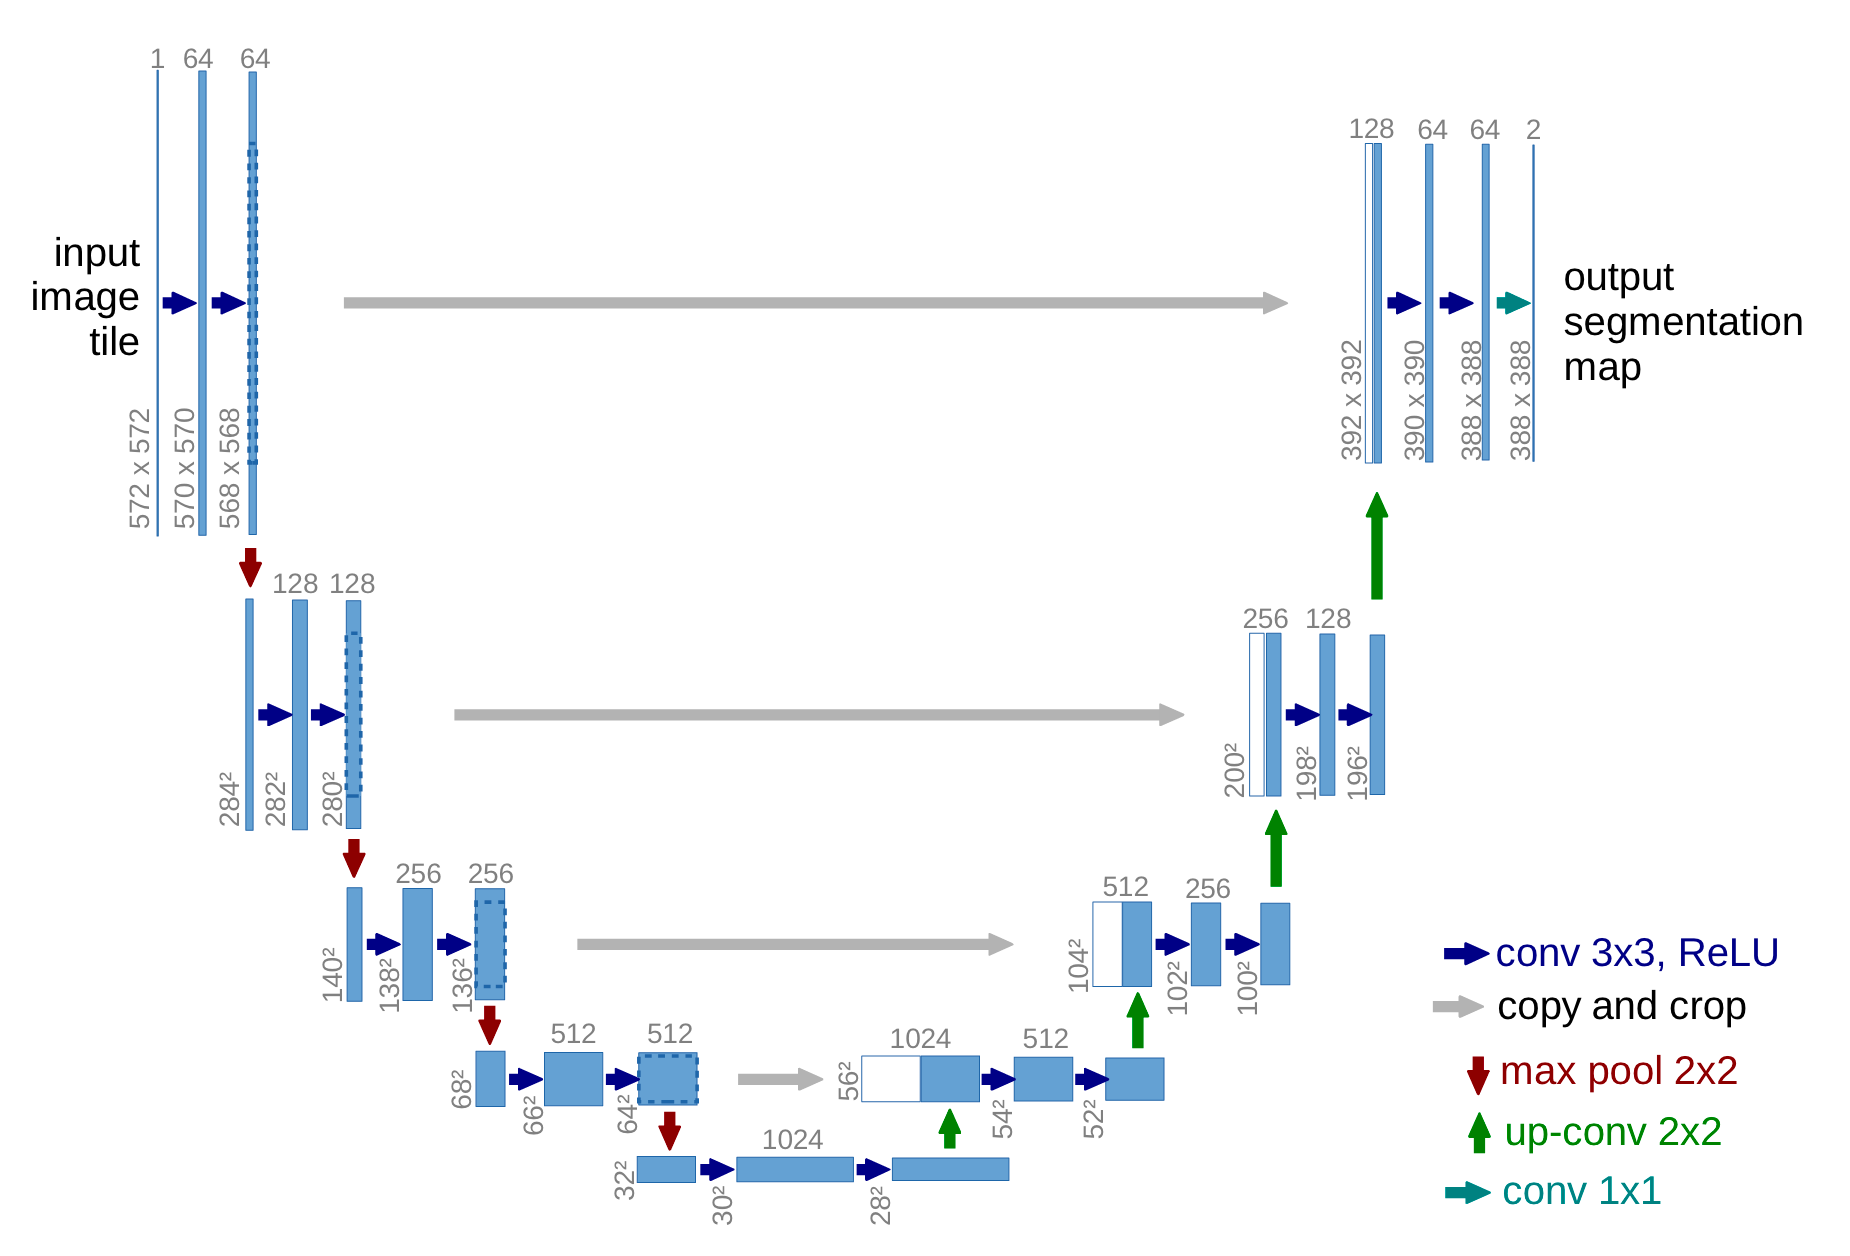
\includegraphics[width=\textwidth]{figures/2-sota/u-net/u-net.png}
    \caption[U-Net]{\textbf{U-Net} --- This figure was taken from the original paper and follows an example for images with $572 \times 572$ pixels. Each blue box corresponds to a multi-channel feature map. The number of channels is denoted on top of the box. The x-y-size is provided at the lower left edge of the box. White boxes represent copied feature maps. The arrows denote the different operations. One can see that at its smallest size, the feature maps were $28 \times 28 \times 1024$, and the end result provides two features maps of $388 \times 388$ pixels, meaning that this specific network could be used, for instance, for segmentation of foreground vs. background. It is also essential to notice that, to keep the original image's fidelity, there is a deconvolutional step for each convolutional one. These are concatenated (represented by the white boxes).}
    \label{fig:u-net}
\end{figure}

The encoder path extracts features from the input image. These features are then compressed into a lower-dimensional representation, which the decoder path uses to generate a segmentation mask for the input image. In this sense, the U-Net architecture can be viewed as a specialized type of \ac{AE} not designed to reconstruct the input image itself.

The U-Net architecture was initially designed to classify each pixel in an image as belonging to a specific object or background: image segmentation. It combines high-level and low-level features from the input image to generate the final segmentation.
\subsubsection{Foundations of Deep Learning} \label{sec:dl-foundations}

This section explores the fundamental principles of \ac{DL}, with a specific focus on activation functions and backpropagation. Activation functions play a vital role in neural networks by introducing non-linearity and enabling the representation of complex relationships. This section covers the most commonly used activation functions. In addition, this section discusses the backpropagation algorithm, which plays a crucial role in training feedforward neural networks by calculating gradients with respect to network weights for iterative adjustments and optimal model performance. Furthermore, this section explores optimization techniques within deep learning.

\paragraph{Activation Functions} \label{sec:activation}

Activation functions are essential to neural networks, as they introduce non-linearity into the model. Nonlinearity is important because it allows the model to learn complex relationships between inputs and outputs. This section will discuss some of the most commonly used activation functions, including sigmoid, \ac{tanh}, and \ac{ReLU}.

\begin{figure}[ht]
    \centering
    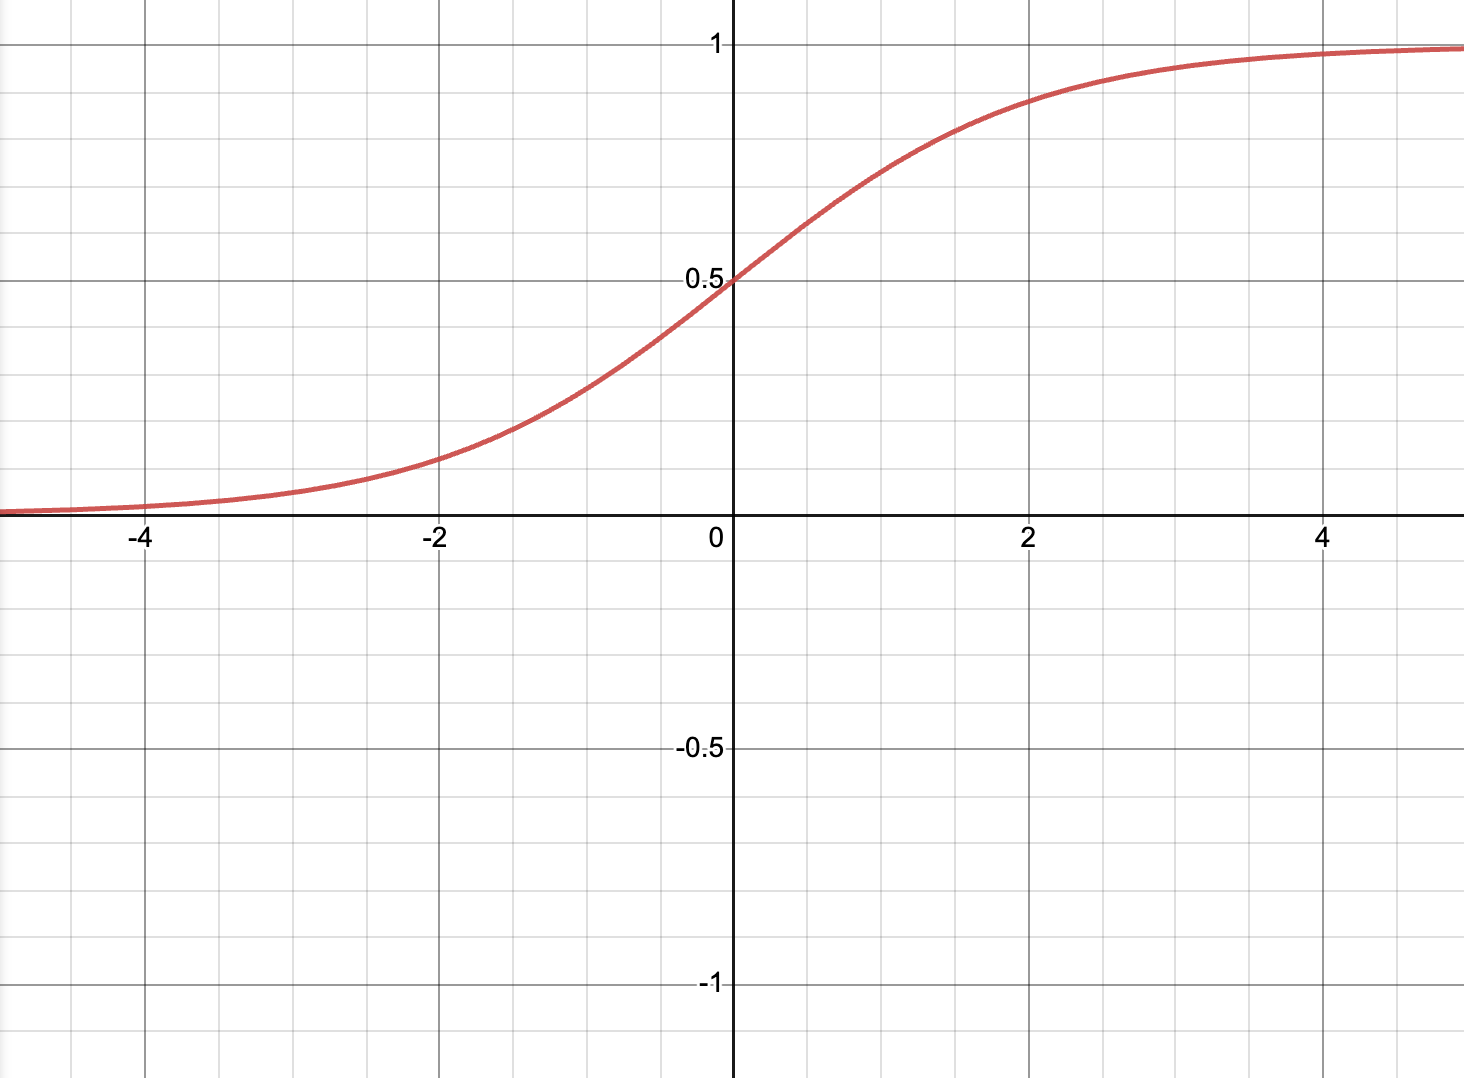
\includegraphics[width=\textwidth/2]{figures/2-sota/activation/sigmoid.png}
    \caption[Sigmoid Activation Function]{One can see that the values that are output are exclusively between 0 and 1 with its value being 0.5 for $x = 0$.}
    \label{fig:sigmoid}
\end{figure}

\label{sec:sigmoid}

The \textbf{sigmoid} activation function is prevalent in neural networks. It is defined as:

\begin{equation}
	\sigma(x) = \frac{1}{1 + e^{-x}}
\end{equation}

where $x$ is the input to the function. The output of the sigmoid function is always between 0 and 1, which makes it useful for binary classification tasks. The sigmoid function is also differentiable, which is essential for backpropagation during training. Figure \ref{fig:sigmoid} visually represents this function.

However, the sigmoid function has a few drawbacks. One issue is that the function's gradient approaches zero as the input becomes very large or very small. This can cause the weights to update very slowly during training, a problem known as the \textit{vanishing gradient} problem. Additionally, the output of the sigmoid function is not zero-centered, which can make optimization more difficult. On the other hand, if the gradients become extremely large, it can cause the weights to update too much in each iteration, leading to the \textit{gradient explosion problem}. This can lead to the model diverging and failing to converge to a good solution. 

\label{sec:tanh}

The \textbf{\acf{tanh}} activation function is similar to the sigmoid function, but its output is between -1 and 1:

\begin{equation}
	\tanh(x) = \frac{e^x - e^{-x}}{e^x + e^{-x}}
\end{equation}

Tanh is differentiable and valuable for binary classification tasks like the sigmoid function. However, it has the same vanishing gradient problem as the sigmoid function. A visual representation can be seen in Figure~\ref{fig:tanh}.

\begin{figure}[ht]
    \centering
    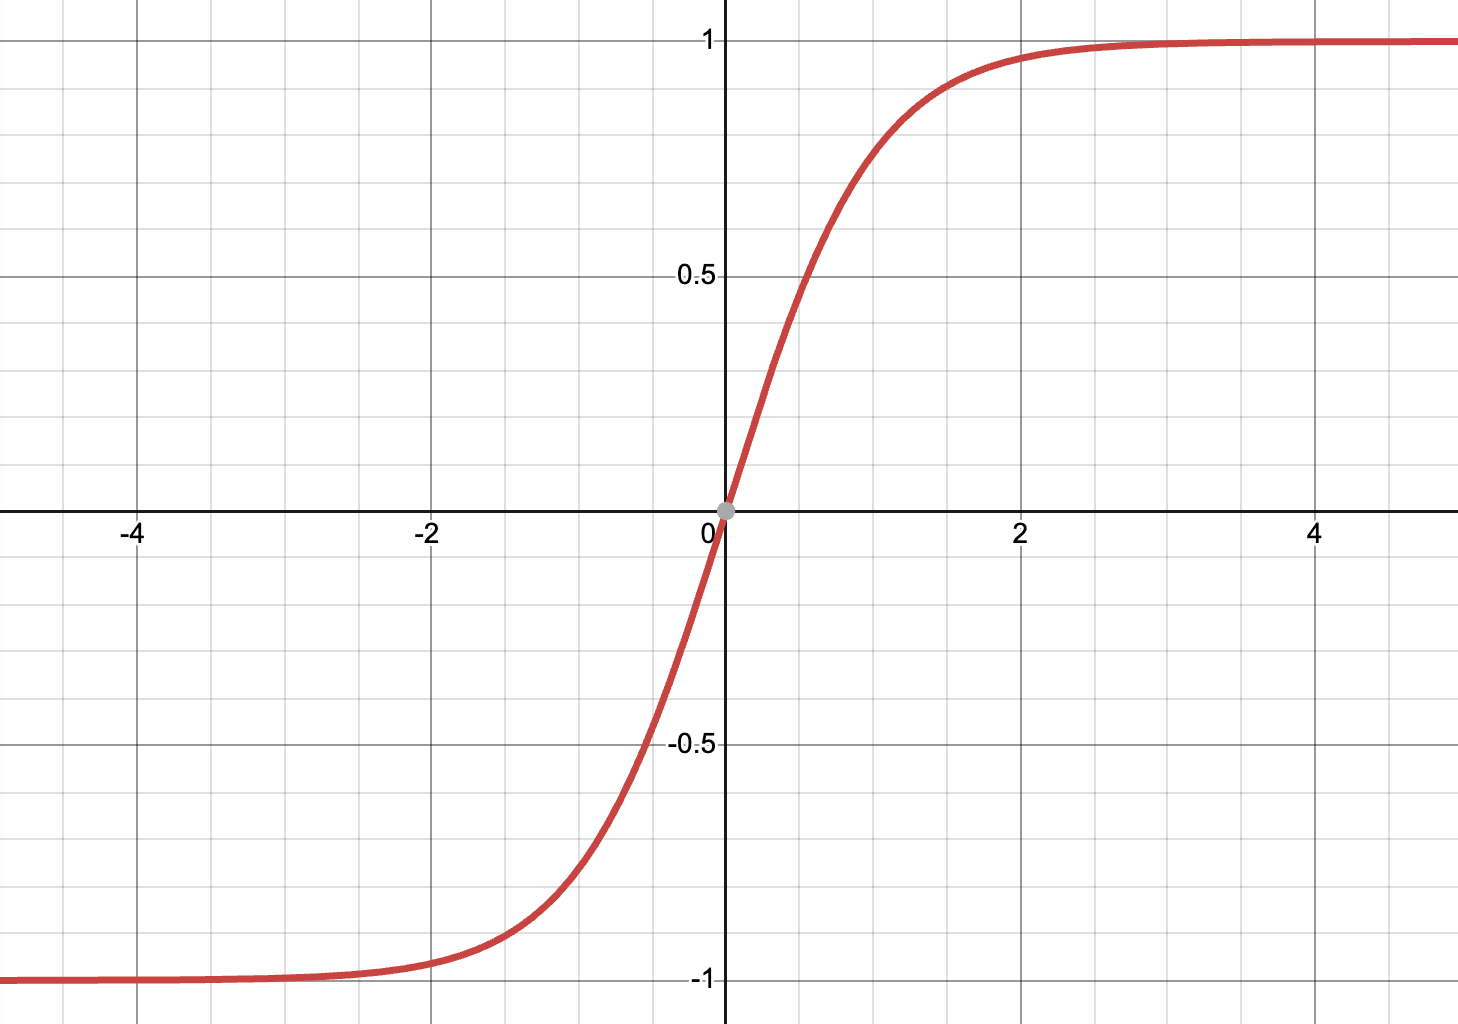
\includegraphics[width=\textwidth/2]{figures/2-sota/activation/tanh.png}
    \caption[Tanh Activation Function]{A very similar function except that its limits are present on -1 and 1}
    \label{fig:tanh}
\end{figure}

\label{sec:relu}

The \textbf{\acf{ReLU}} activation function is a popular choice in \ac{DL}. It is defined as:

\begin{equation}
	\text{ReLU}(x) = \max(0, x)
\end{equation}

The \ac{ReLU} function is also zero-centered, which can make optimization easier. However, this function is not differentiable at $x=0$, which can cause problems during training. Variants of the \ac{ReLU} function have been proposed to address this issue. A visual representation can be seen in Figure \ref{fig:relu}.

\begin{figure}[ht]
    \centering
    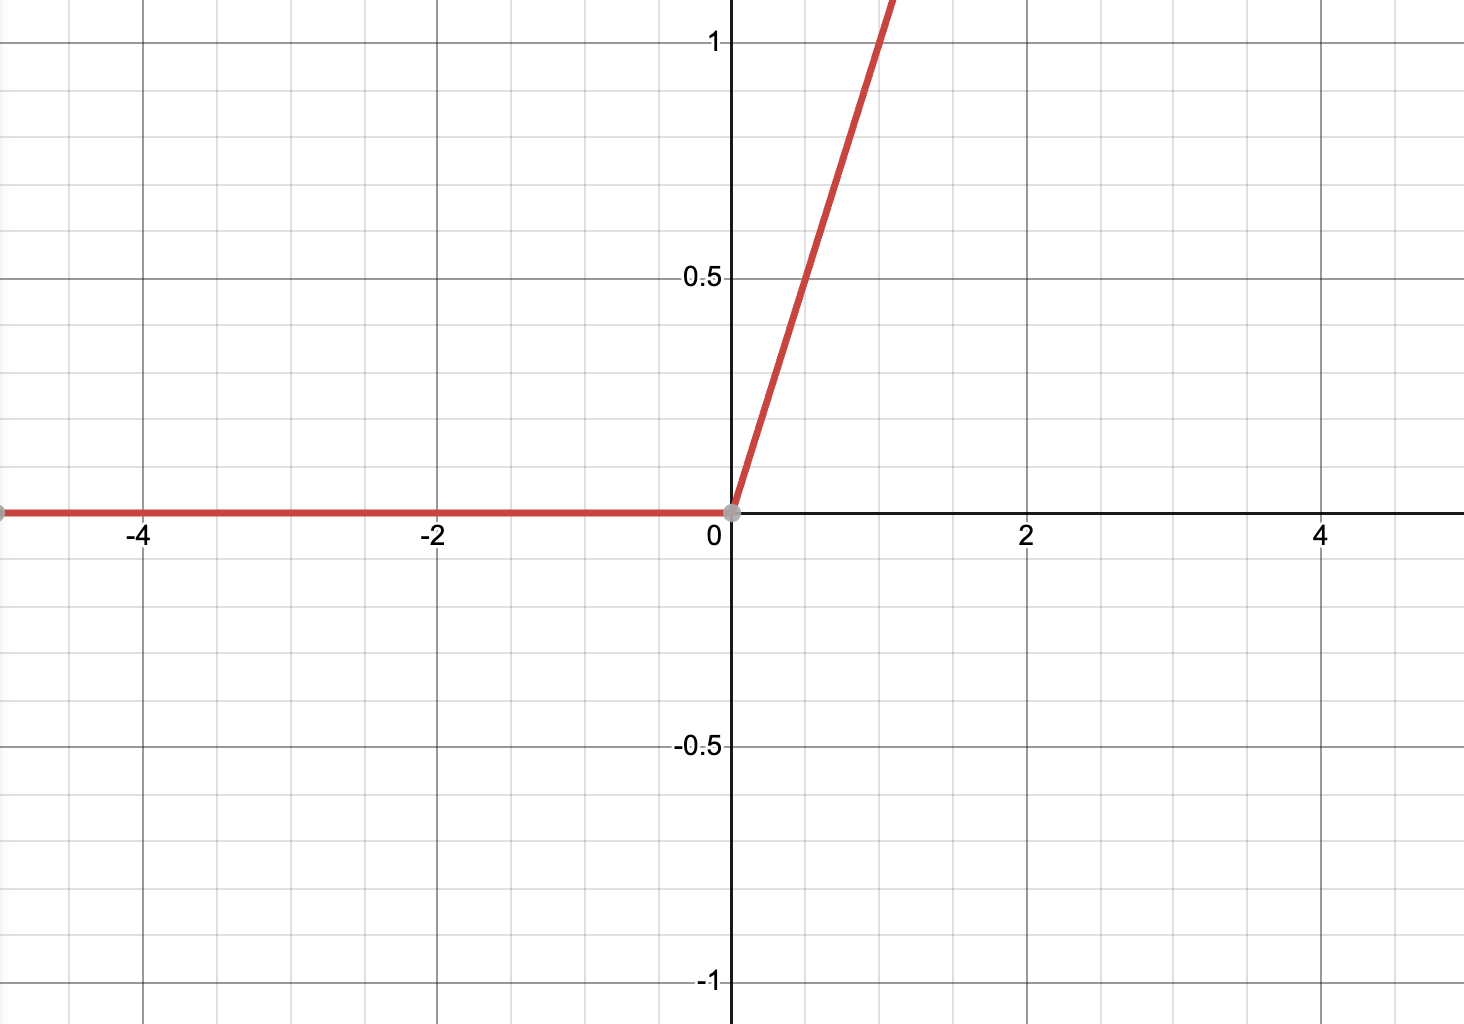
\includegraphics[width=\textwidth/2]{figures/2-sota/activation/relu.png}
    \caption[Relu Activation Function]{Linear for positive values, 0 for negative values.}
    \label{fig:relu}
\end{figure}

The \ac{ReLU} activation has a potential problem known as the \textit{dying ReLU} problem. When a neuron's weights become such that its input is always negative, its gradient will always be zero. In this situation, the neuron will become inactive, or \textit{dead}, and will no longer update during training. This problem can lead to underfitting, as some neurons stop learning and contributing to the model. Variants of \ac{ReLU}, such as \textbf{Leaky \ac{ReLU}}, have been proposed to mitigate the dying \ac{ReLU} problem by assigning a slight non-zero gradient for negative input values.

The Leaky ReLU function is defined as:

\begin{equation}
\text{Leaky ReLU}(x) = \text{max}(a x , x)
\end{equation}

where $a$ is a small positive number such as $0.01$. This non-zero gradient for negative inputs can help prevent neurons from becoming inactive during training. This function can visually be seen in Figure~\ref{fig:leaky-relu}.

\begin{figure}[ht]
    \centering
    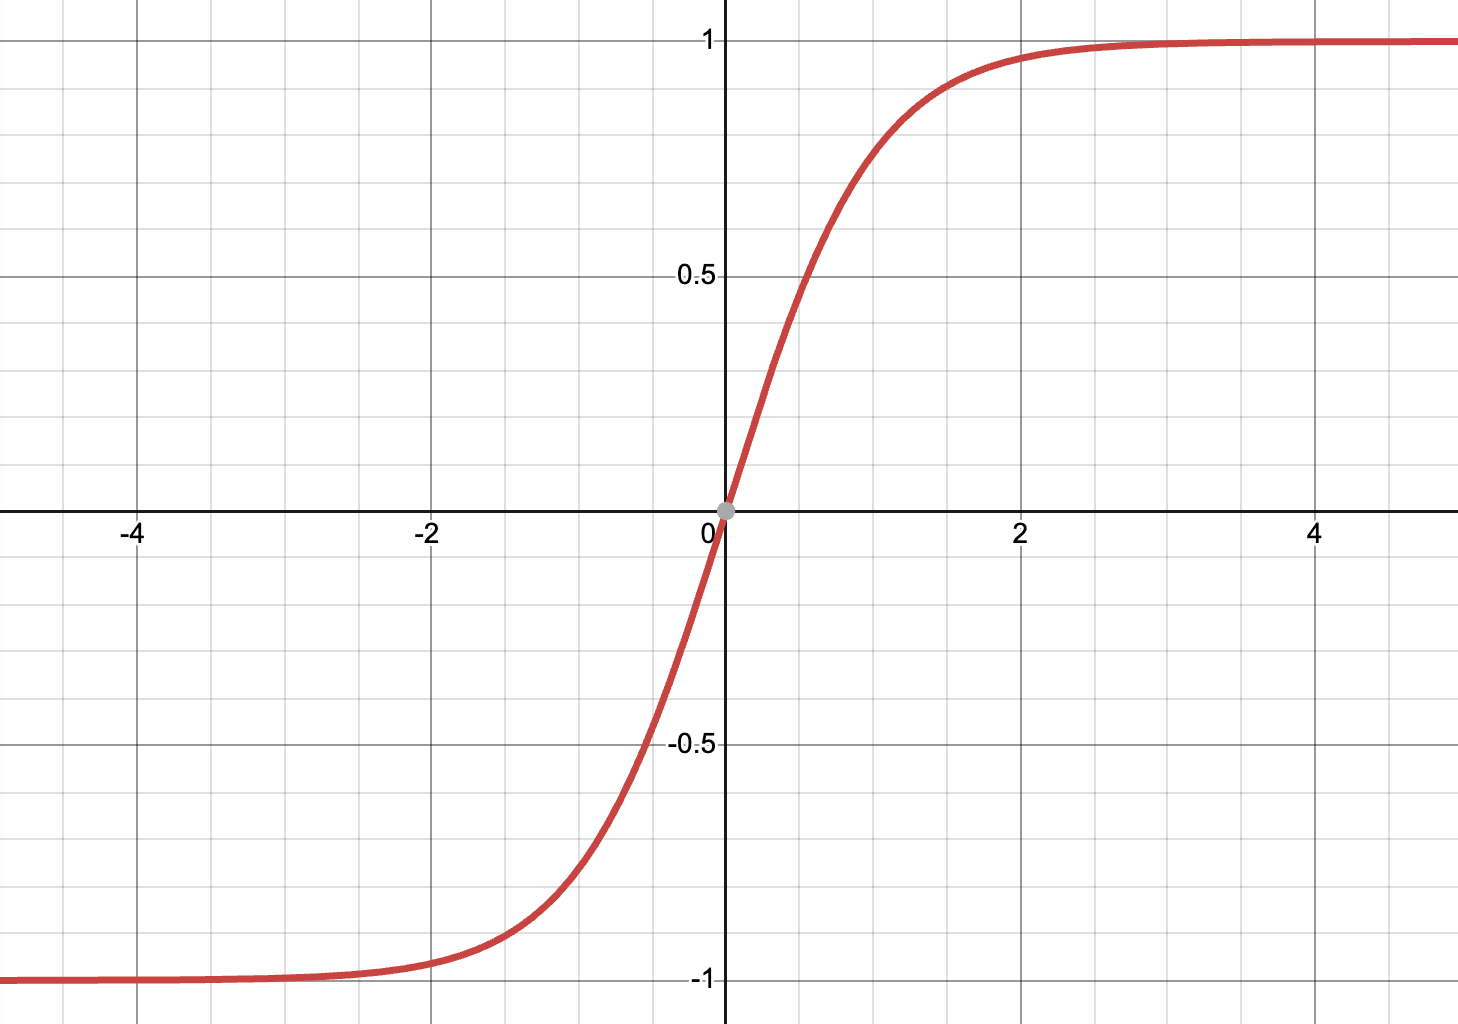
\includegraphics[width=\textwidth/2]{figures/2-sota/activation/tanh.png}
    \caption[Leaky Relu Activation Function]{Very similar to Relu but with non-zero gradient for negative inputs.}
    \label{fig:leaky-relu}
\end{figure}
\paragraph{Backpropagation Algorithm for Training Neural Networks} \label{sec:backpropagation}

\textit{Backpropagation} is an algorithm used to train feedforward neural networks by computing the gradient of the loss function concerning the network weights. This gradient is then used to update the weights in the opposite direction of the gradient, allowing the network to learn how to predict outputs given inputs accurately.

To understand backpropagation, it is crucial to define the loss function, which measures the network's performance on a given task. For instance, the cross-entropy loss is commonly used in classification tasks to quantify the difference between predicted probabilities and the correct labels. More information on loss functions can be found in Section \ref{sec:loss-functions}. Backpropagation adjusts the network weights to minimize the loss function.

The backpropagation algorithm works by computing the gradient of the loss function concerning each weight in the network. This gradient tells how much the loss function would change if one were to make a small change to the weight. This gradient is then used to update the weight in the direction that reduces the loss function.

The gradient is computed using the chain rule of calculus. Considering a simple feedforward neural network with one hidden layer. The output of the network is given by:

\begin{equation}
	y = h(\sum_{j=1}^M w_{2,j} h(\sum_{i=1}^N w_{1,i} x_i + b_1) + b_2)
\end{equation}

where $x_i$ is the $i$-th input, $w_{1, i}$ and $w_{2, j}$ are the weights connecting the input to the hidden layer and the hidden layer to the output, respectively, $b_1$ and $b_2$ are the biases of the hidden layer and the output, respectively, $h$ is the activation function, such as sigmoid, (see section \ref{sec:activation}), and $N$ and $M$ are the numbers of inputs and hidden units, respectively.

The loss function is a function of the output $y$ and the actual label $t$.

To compute the gradient of the loss function concerning a weight $w_{i,j}$, one first needs to compute the local gradient of the output for the weight. This is given by:

\begin{equation}
	\frac{\partial y}{\partial w_{i,j}} = h'(\sum_{j=1}^M w_{2,j} h(\sum_{i=1}^N w_{1,i} x_i + b_1) + b_2) h(\sum_{i=1}^N w_{1,i} x_i + b_1) w_{2,j}
\end{equation}

where $h'$ is the derivative of the activation function. One can then use the chain rule to compute the gradient of the loss function for the weight:

\begin{equation}
	\frac{\partial E}{\partial w_{i,j}} = (y - t)\frac{\partial y}{\partial w_{i,j}}
\end{equation}

Once one has computed the gradient of the loss function concerning all the weights in the network, the weights can be updated using gradient descent:

\begin{equation}
	w_{i,j} \leftarrow w_{i,j} - \alpha \frac{\partial E}{\partial w_{i,j}}
\end{equation}

where $\alpha$ is the learning rate, which determines the step size of the weight update.

Backpropagation can be extended to networks with multiple hidden layers using the chain rule to propagate the gradient backward through the network.
\paragraph{Optimization with Stochastic Gradient Descent} \label{sec:sgd}

\Acf{SGD} is a widely used optimization algorithm in \ac{DL}. It is an iterative method that minimizes the loss function by updating the model parameters in the direction of the negative gradient of the loss function. In each iteration, \ac{SGD} randomly selects a subset of the training data, called a mini-batch, and computes the gradient of the loss function concerning the parameters using the mini-batch. The parameters are then updated by subtracting the product of the gradient and a learning rate hyperparameter, which controls the step size of the update. The learning rate is typically set to a small value to ensure the stability and convergence of the algorithm.

Technically, it would be possible to use the loss of all the samples to update the model weights. However, using all the samples to update the weights, also known as batch gradient descent, can be computationally expensive and memory-intensive, especially for large datasets. In contrast, \ac{SGD} updates the weights based on a randomly selected sample mini-batch, reducing the computational and memory requirements and enabling faster convergence.

Moreover, \ac{SGD} introduces stochasticity in the optimization process, which can help the algorithm escape from local minima and explore different regions of the parameter space. This can improve the model's generalization performance and prevent overfitting the training data.

However, \ac{SGD} can also be noisier and less stable than batch gradient descent due to the mini-batches random sampling and the gradients' fluctuation. Therefore, finding an appropriate learning rate and mini-batch size is crucial for the solutions' convergence and quality in \ac{SGD}.

Formally, let $\theta$ be the vector of model parameters, $L(\theta)$ be the loss function, $D$ be the training dataset, and $B$ be a mini-batch sampled from $D$. Then, the update rule for \ac{SGD} can be written as:

\begin{equation}
	\theta_{t+1} = \theta_{t} - \alpha \nabla_{\theta} L(\theta_t; B)
\end{equation}

where $\alpha$ is the learning rate, and $\nabla_{\theta} L(\theta_t; B)$ is the gradient of the loss function concerning the parameters evaluated on the mini-batch $B$ at iteration $t$.

\ac{SGD} has several advantages, such as its simplicity and low memory requirements, which make it suitable for large-scale datasets and complex models. However, it also has some limitations, such as its sensitivity to the learning rate and the mini-batch size, which can affect the solutions' convergence and quality. Therefore, several variants of \ac{SGD}, such as Adagrad (that adapts the learning rate for each parameter based on its historical gradients, working well for sparse data) and Adam (explained in Section \ref{sec:adam}, adds a fraction of the previous update to the current update, and adapts the learning rate), have been proposed to address these issues and improve the algorithm's performance.
\paragraph{Optimization with the Adam Optimizer} \label{sec:adam}

Adam is a variant of \ac{SGD} (see Section \ref{sec:sgd}) that adapts the learning rate for each parameter based on the estimates of the first and second moments of the gradients \cite{kingma_adam_2017}.

Adam addresses some of the limitations of \ac{SGD}, such as the sensitivity to the learning rate and the mini-batch size, using a more sophisticated update rule incorporating information about the gradients and their history. Specifically, Adam computes a moving average of the gradients and their squares, which adjusts the updates' learning rate and momentum.

The estimates of the moments are computed as follows:

\begin{equation}
    m_t = \beta_1 m_{t-1} + (1-\beta_1)g_t
\end{equation}

\begin{equation}
    v_t = \beta_2 v_{t-1} + (1-\beta_2)g_t^2
\end{equation}

where $g_t$ is the gradient of the loss function with respect to the parameters at iteration $t$, $m_{t-1}$ and $v_{t-1}$ are the estimates of the moments at the previous iteration, and $\beta_1$ and $\beta_2$ are the decay rates for the moving averages of the gradients and their squares, respectively.

The update rule for Adam can then be written as follows:

\begin{equation}
    \theta_{t+1} = \theta_{t} - \frac{\alpha}{\sqrt{\hat{v}_t+\epsilon}}\hat{m}_t
\end{equation}

where $\theta_t$ is the vector of model parameters at iteration $t$, $\alpha$ is the learning rate, $\hat{m}_t$ and $\hat{v}_t$ are the biased estimates of the first and second moments of the gradients, respectively, and $\epsilon$ is a small constant to avoid division by zero.

The biased estimates of the moments are computed as follows:

\begin{equation}
    \hat{m}_t = \frac{m_t}{1-\beta_1^t}
\end{equation}

\begin{equation}
    \hat{v}_t = \frac{v_t}{1-\beta_2^t}
\end{equation}

where $t$ is the iteration number. The bias correction is necessary to account for the fact that the estimates are initialized at zero and may be biased towards zero in the early iterations.

By using the biased estimates of the moments, Adam can handle noisy or sparse gradients and converge faster than SGD on a wide range of optimization problems. However, the choice of the hyperparameters, such as the learning rate, the decay rates, and the epsilon value, can significantly affect the performance of Adam and should be carefully tuned for each problem.

Adam combines the benefits of both momentum and adaptive learning rates by using the moving average of the gradients to update the momentum and the moving average of the squared gradients to adapt the learning rate. Unlike \ac{SGD}, which uses a fixed learning rate for all parameters, Adam adapts the learning rate individually for each parameter based on the estimate of the second moment of the gradient. This can improve the solutions' convergence and quality, especially for problems with sparse or noisy gradients. Moreover, Adam can handle non-stationary objective functions and noisy gradients, which can be challenging for other optimization algorithms.

However, Adam also has some limitations, such as its sensitivity to the choice of hyperparameters and its tendency to overshoot the optimal solution. Therefore, tuning the hyperparameters carefully and monitoring the algorithm's convergence during training is important.
\subsubsection{Generative Deep Learning Architectures}

Generative \ac{DL} architectures are a subset of \ac{DL} networks designed to generate new and diverse data samples from a learned distribution.

By finding latent data structures and learning to reproduce the hidden statistics behind observed data, they do so. To achieve this, the model tries to estimate an underlying probability distribution $p_{data}$ when given a set of samples from this distribution. Thus, training a generative model involves selecting the best parameters that reduce some concept of distance/loss/error between the model and the actual distribution. As Huzaifah \cite{huzaifah_deep_2021} states: ``given training data points $X$ as samples from an empirical distribution $p_{data}(X)$, we want to learn a model $p_\theta(X)$, belonging to a model family $M$ that closely matches $p_{data}(X)$, by repeatedly changing model parameters $\theta$''. This is expressed as the problem in equation \ref{eq:generative-models-base}.

\begin{equation} \label{eq:generative-models-base}
    \min_{\theta \in M} d (p_{data}, p_\theta)
\end{equation}

Standard functions for $d$ are displayed in section \ref{sec:loss-functions}.

These models have been applied to various tasks, such as image synthesis, text generation, and audio synthesis. Generative \ac{DL} models have gained popularity recently due to their ability to produce high-quality data and model complex distributions.

This section will present the most used architectures.

\paragraph{Deep Autoregressive Network (DARN)} \label{sec:darn}

First introduced in 2013, \acf{DARN} is an architecture for generative models that are used to generate data by using an \acf{AR} approach \cite{gregor_deep_2014}.

\Ac{AR} models generate data by predicting the following sample in a sequence based on the previous samples. In the case of \acp{DARN}, the model has multiple hidden layers to do so. The idea behind it is to model the data's complex, high-dimensional probability distribution by breaking it down into a series of simple, conditionally independent distributions. This is done by learning a deep neural network that maps inputs to outputs through a series of hidden layers. This allows the network to build up a complex representation of the data distribution over time, capturing complex patterns in the data and ultimately making more precise predictions.

By applying the chain rule of probability, \ac{AR} models can create a feasible density model that breaks down the probability distribution over $n$ time steps \cite{huzaifah_deep_2021}, as shown in equation

\begin{equation} \label{eq:chain-rule}
    p(X) = \prod_{i=1}^n p(x_i|x_1, ..., x_{i-1})
\end{equation}

This method implies that data has a standard sequential order—the present term in the sequence $(x_i)$ depends only on a recent window of preceding terms. Future terms are not taken into account. This is, ultimately, they assume that a data point only depends on previous ones and learn to predict the following sample is given only what has come just prior. The rationale behind this technique is similar to the one that \acp{RNN} employ. In fact, an \ac{RNN} can be seen as an \ac{AR} model that reduces the previous terms to a hidden state rather than giving them directly as input to a layer \cite{huzaifah_deep_2021}. Besides, \ac{AR} models are more straightforward and faster to train. Indeed, an \ac{AR} model is a feedforward model (see Section \ref{sec:feedforward} )which predicts future values from past values. One can imagine a model similar to a feedforward neural network that is not fully connected but with only some connections regarding past inputs. This can be seen in Figure \ref{fig:darn}.

\begin{figure}[ht]
    \centering
    \ctikzfig{figures/2-sota/darn}
    \caption[Deep autoregressive network]{\textbf{\Acf{DARN}} --- The input of each neuron in a given layer is conditioned by the output of the 2 previous neurons in the previous output.}
    \label{fig:darn}
\end{figure}
\paragraph{Variational Autoencoder (VAE)} \label{sec:vae}

Kingma and Welling proposed the concept of \acfp{VAE} in 2013 \cite{kingma_auto-encoding_2022}. The authors proposed a new approach to traditional \acp{AE} that utilizes a variational inference method to model complex distributions in high-dimensional spaces. Thus allowing for the generation of new, unseen data similar to the initial training.

In the realm of \acp{AE}, traditional approaches, as discussed in Section \ref{sec:autoencoders}, aim to map the identity function through the utilization of encoder and decoder networks. The encoder takes the input and transforms it into a compressed vector representation, while the decoder reconstructs the input from this compressed representation. However, Variational Autoencoders (\acp{VAE}) introduce a distinct variation in their approach. Instead of modeling the input as a deterministic vector, the encoder in \acp{VAE} characterizes the input data as a probability distribution across potential representations. This distribution is typically represented by two sets of latent values: one corresponding to the mean and the other to the variance. These latent sets are often modeled using fully connected layers within the architecture.

Consequently, the \ac{VAE} framework imposes a constraint on the embedded vector by confining it to a specified number of points in a hyperplane. Interestingly, this enables us to discard the encoder entirely. By working with a continuous latent space, the decoder of the \ac{VAE} can generate novel and diverse samples akin to the training data. Figure \ref{fig:vae} provides a visual depiction of this concept, illustrating how the decoder operates based on samples from the latent distribution to generate new output.

\begin{figure}[ht]
    \centering
    \ctikzfig{figures/2-sota/vae}
    \caption[Variational autoencoder]{\textbf{\Acf{VAE}} --- The \ac{VAE} encoder operates in a manner comparable to the traditional \ac{AE}, but with a notable distinction. Instead of directly mapping the input to a single latent representation, the \ac{VAE} encoder translates the input into two sets of latent features: the normals and the variances. These latent features are represented in the Figure by the two sets of nodes within the bottleneck of the encoder architecture.}
    \label{fig:vae}
\end{figure}

This was encouraging, as distributions near each other would produce similar outputs. This means, it created smooth changes between data points. The explanation for this is that \acp{VAE} discover low-dimensional parameterized representations of the data \cite{huzaifah_deep_2021}.

For training, these networks use an objective function that aims to minimize the loss between input and output and ensure that the learned distribution is similar to a prior distribution, such as a Gaussian.

However, sometimes during training, the \ac{VAE} can learn to ignore the latent variable and instead rely solely on the decoder network to generate the output. This means that the encoder network outputs the same distribution over the latent space for all input data points, resulting in a collapsed posterior distribution. In other words, the encoder fails to capture the variability in the input data, and the decoder generates outputs that are not diverse.

This phenomenon is known as \textit{posterior collapse}, and it can occur due to various reasons, such as a high reconstruction loss weight or a small latent space size. Posterior collapse can severely impact the performance of the \ac{VAE} and result in poor-quality generated samples.

These models can be used for any generative task, such as computer vision, natural language processing, and sound generation.

\paragraph{Generative Adversarial Network (GAN)} \label{sec:gan}

The paper ``Generative Adversarial Networks'' by Goodfellow et al. \cite{goodfellow_generative_2014} introduced a novel framework for generative modeling using deep neural networks. The main idea behind \acp{GAN} is to train two neural networks simultaneously, one generator and one discriminator.

By transforming a random noise vector $z$ into a target distribution in some data space $\hat{X}$ (for example, spectrograms), the generator network $G$ produces new samples. Meanwhile, the discriminator $D$ attempts to tell apart synthetic and real data; that is, $D$ assigns the input data, whether it is $X$ or $\hat{X}$, a categorical label based on whether it believes the input originated from the actual data distribution $p(X)$ or the model distribution $p(z)$. Figure \ref{fig:gan} shows this process.


\begin{figure}[ht]
    \centering
    \ctikzfig{figures/2-sota/gan}
    \caption[Generative adversarial network]{\textbf{\Acf{GAN}} --- A random noise vector $\vec{z}$ is passed through the generator in $G(\vec{z})$ to create the synthetic sample $\hat{X}$. Both this and the real sample $X$ are passed to the discriminator $D$ that predicts which of the samples is the real one. It is important to notice that in this illustration, the circles represent entire neural networks and not simply neurons.}
    \label{fig:gan}
\end{figure}

Using a minimax optimization framework, the networks are trained in an adversarial way. The goal is that $G$ generates a fake sample $\hat{X}$ that is given to $D$ along with a real one $X$. This network then has to identify which is genuine and which is fabricated. $D$ is trained to increase the probability of telling apart the real from the fake data. While $G$ is trained at the same time for the opposite objective, that is, to deceive $D$ by minimizing $\log(1 - D(G(z)))$ \cite{huzaifah_deep_2021}. $G$ and $D$ are trained in turns until a Nash equilibrium is achieved.

When $G$ creates flawless fake data that cannot be told apart from real data, a Nash equilibrium is reached. $D$ has no clue whether the data is real or fake and just makes random guesses about the input label. In this situation, $G$ performs at its best, and $D$ performs at its worst. The models cannot get any better than this. This is a perfect scenario that requires effort to attain in reality. It is worth noting that the generator never sees the training samples, only the feedback given by the discriminator \cite{huzaifah_deep_2021}.

Once the training is done, the discriminator is thrown away, and the generator can be used to draw samples from the learned distribution of the real data. The generator has learned to associate random vectors with data samples in the target domain. These vectors usually represent some features. As a result, they cluster output data with similar features to nearby input values, offering a natural way of exploring output data with different attributes. This implies that similar input vectors will produce similar outputs \cite{huzaifah_deep_2021}.

Although this technique has seen great success in producing high-resolution images, it still needs to improve in the audio domain as the sections in Section~\ref{sec:related-work} show. Besides that, even in ideal settings, it has some drawbacks. For instance, the fact that the training of the whole model implies the training of two different networks makes it unstable. It is easy to get stuck at a sub-optimal nash equilibrium. One such example is mode collapse, where the generator produces limited variations of the target distribution.

\Acfp{DARN} (see Section \ref{sec:darn}) represented the state-of-the-art in neural audio synthesis for a long time. These models are good at learning local latent structure, this is, the features of sounds over brief periods. However, they struggle with longer-term features. Besides, \acp{DARN} are very slow because they generate waveforms one sample at a time. \Acp{GAN} are capable of modeling global latent structure since they build the output as a whole; moreover, after training, they generate way faster \cite{tahiroglu_-terity_2020}, showing promising features for audio generation.
\paragraph{Normalizing Flow Models} \label{sec:flow-model}

Normalizing flow models provide a flexible and robust framework for generative modeling and were first introduced in 2015 \cite{rezende_variational_2016}.

The main idea is to use the change of variables in the probability distributions technique to convert simple distributions into more complicated ones. This technique requires applying a transformation to a distribution that changes it into another, more intricate, distribution. The entire idea begins with a simple distribution (for instance, Gaussian) for a set of hidden variables $z$. The goal is to change this distribution into a complex one that corresponds to an output $X$. A single transformation is provided by a smooth and reversible function $f$ that can relate $z$ and $X$, such that $X = f (z)$ and $z = f^{- 1}(X)$. Considering the complexity of $X$, one of these transformations might not produce a sufficiently complex distribution. Hence, multiple reversible transformations are combined sequentially, forming a ``flow''. Neural network layers determine each mapping function in the flow \cite{huzaifah_deep_2021}. Figure \ref{fig:normalizing-flows} illustrates this process.

\begin{figure}[ht]
    \centering
    \ctikzfig{figures/2-sota/normalizing-flows}
    \caption[Normalizing flows network]{\textbf{Normalizing flows network} --- This illustration was based on \cite{weng_flow-based_2018} and shows the application of multiple invertible functions $f_k$ composed one after the other in order to build the complex output $z_K = x$ from a simple Gaussian distribution.}
    \label{fig:normalizing-flows}
\end{figure}

Accurately, let $z_0$ be a multivariate random variable with a distribution $p_0(z_0)$ where $p_0$ is, for example, a Gaussian distribution. Then, for $i = 1, ..., K$ where $K$ is the number of flow operations, let $z_i = f_i(z_{i - 1})$ be a sequence of random multivariate variables. $f_i^{-1}$ should exist for training to occur. The final output $z_K$ models the target distribution.

Normalizing flow models are flexible, meaning they can model various distributions by stacking multiple normalizing flows to form a deep network. This allows it to capture complex relationships between variables in the data.

These models have been proven effective for the generative modeling of high-dimensional data.

In the generative scene, these models are distinguished from the previously mentioned ones because they can speed up the generations and modeling processes \cite{huzaifah_deep_2021}.
\paragraph{Diffusion Models} \label{sec:diffusion}

Until the proliferation of diffusion models, the architecture most used for data generation was the \ac{GAN} (Section \ref{sec:gan}). The problem is that \acp{GAN} are hard to train. For instance, mode collapse can happen. In mode collapse, the generator always generates the same data that fools the discriminator.

\textit{Diffusion models} \cite{sohl-dickstein_deep_2015} simplify this generation process into more intuitive small steps where the work of the network is lighter and is run multiple times. This is done by taking inspiration from non-equilibrium thermodynamics. These models define a Markov chain of diffusion steps to slowly add random noise to data and then learn to reverse the diffusion process to construct desired data samples from the noise.

Practically, diffusion models use a Markov chain to gradually convert one distribution into another. This chain starts from a simple known distribution (\textit{e.g.} a Gaussian) into a target distribution using a diffusion process. Learning in this framework involves estimating small perturbations to a diffusion process, using a network such as the U-Net (Section \ref{sec:u-net}). Estimating small perturbations is more tractable than explicitly describing the whole distribution with a single, non-analytically-normalizable potential function. This process can be seen in Figure \ref{fig:diffusion}

\begin{figure}[ht]
    \centering
    \ctikzfig{figures/2-sota/diffusion}
    \caption[Diffusion model]{\textbf{Diffusion model} --- This illustration was based on \cite{ho_denoising_2020} and shows the process of applying Gaussian noise to an image sample through multiple steps $q(X_t|X_{t-1})$. The model will then learn the operation $p$ that transforms $X_t$ into $X_{t-1}$ with $p(X_{t-1}|X_t)$ and so on until $X_0$. At this point, the model has generated a new data sample.}
    \label{fig:diffusion}
\end{figure}

The ultimate goal is to define a forward (or inference) diffusion process which converts any complex data distribution into a simple, tractable distribution and then learn a finite-time reversal of this diffusion process which defines the generative model distribution \cite{sohl-dickstein_deep_2015}.

One problem is that one needs to decide how much noise one wants to increment per iteration. For instance, if one decides to train a network that directly learns to denoise full Gaussian to a real image, then one is simply training a \ac{GAN} generator. It is easier to remove a small amount of noise per iteration. The amount of noise added per iteration is a hyperparameter called a scheduler. For instance, one can add the same amount of noise per iteration, called the \textit{linear schedule}. Multiple schedules may have different impacts.

For instance, given a linear scheduler, one can define that for $t = x$, the sample would be the original one with $k = x \times 10$ random data points with Gaussian noise. This allows data generation in different timestamps without running through all timestamps. For instance, generating a data sample with $t = 5$ would be as easy as noising $k = 50$ random data points.

To train these networks, one would give pairs of the original data sample $X$ plus a data sample at a random timestamp $X_t$ plus the random step $t$, $X_t = X + N(t)$ where $N$ is a noising function. The network would learn to get the noise from the data given a timestamp. This means that the network would learn to predict $N(t)$ using image segmentation. This will not always be perfect, so the network learns to predict $\tilde{N(t)}$. Then, theoretically, by applying $X_t - \tilde{N(t)}$, one gets $\tilde{X}$, which should be as close as possible to $X$. This process for $t = 50$ is challenging, as most of the data is Gaussian noise. However, applying the process for, for instance, $t = 1$, should be quite easy.

For inference, one gets noisy data $X_t$ and a given timestamp $t$. Applying the network returns $\tilde{N(t)}$ as explained previously. By doing $\tilde{X} = X_t - \tilde{N(t)}$, one generates a bad data sample. But then, the algorithm takes $\tilde{X}$ and applies $N(t - 1)$. This results in another noisy data sample with less noise. This process loops until $t = 0$. By then, a new data sample is generated.
\paragraph{Transformers} \label{sec:transformers}

In 2017, the introduction of the ``Attention is All You Need''~\cite{vaswani_attention_2017} paper marked a significant milestone in \ac{DL}. Although initially introduced for \ac{NLP}, the transformer architecture has proven helpful in various data generation tasks, including audio synthesis as shown in Section~\ref{sec:related-work}. This marked a paradigm shift from the conventional \ac{RNN}-based models, which were earlier widely used, with some incorporating a rudimentary form of the attention mechanism.

In transformers, attention is a key component that allows the model to focus on relevant parts of the input sequence when making predictions. Mathematically, attention can be defined as a weighted sum of values based on their importance or relevance.

Let's break down the mathematical formulation of attention in transformers:

Query \(Q\), Key \(K\), and Value \(V\): These are three linear transformations applied to the input sequence. The query represents the element for which we want to compute attention weights, while keys and values represent all elements in the sequence.

To calculate how much each value contributes to the output for a given query, we compute dot products between the query and all keys:

\begin{equation}
    \text{{scores}} = Q \cdot K^T
\end{equation}

Here, \(\cdot\) represents matrix multiplication, \(K^T\) denotes transpose of matrix \(K\).

The next step is to normalize these scores using a softmax function along dimension 1 (rows) to obtain attention weights that sum up to 1:

\begin{equation}
    \text{{weights}} = \text{{softmax}}(\text{{scores}})
\end{equation}

Finally, we take a weighted sum of values using these normalized attention weights:

\begin{equation}
\begin{split}
    &\text{{attended\_values}} = V \cdot {\text{{weights}}} \\
    &\text{{output}} = {\sum{( {\text{attended\_values} } })}
\end{split}
\end{equation}

Here, $\text{softmax}$ computes exponentiated values scaled by their row-wise sums, while $\text{sum}$ performs summation across rows.

The resulting output represents an attended representation obtained by giving higher weightage/importance to more relevant parts of the input sequence based on similarity with respect to the query. This mathematical formulation allows transformer models to capture long-range dependencies effectively by attending to the pertinent information in the source sequence when generating predictions.

The attention mechanism allows the model to give different importance to different input parts. For instance, let us imagine a translation task English-Portuguese. If naively translated, the sentence ``She is a doctor'' could be translated to ``Ela é um doutor''. However, if, when generating the last word, the model gives some importance to the word ``she'', it might guess that the correct word is ``doutora''.

The key idea behind transformers is to completely disregard the recurrent architecture and only use attention by using self-attention. Self-attention is a mechanism that allows the calculation of the importance of each input element concerning all other elements in the input sequence. This allows the model to dynamically focus on the most relevant information at each step of the calculation instead of relying on fixed relationships between elements in the input as in traditional recurrent neural networks.


%% HERE
The transformer architecture, shown in Figure \ref{fig:transformer}, serves as the basis for advanced transformers utilized in a variety of applications, such as audio synthesis. This architecture includes an encoder and decoder, both with stacked layers, which are essential to processing textual input data and producing consistent audio waveforms.

The encoder, consisting of $N$ identical layers, aims to convert the input text into continuous representations that encapsulate crucial semantic information. Each layer features two sub-layers that enable this conversion:

\begin{enumerate}
    \item Multi-Head Self-Attention: As explained above, this mechanism allows the encoder to model input text sequence dependencies objectively. Multiple scaled dot-product attention heads attend to various positions of the text sequence simultaneously. This process captures intricate relationships within the text in parallel, enriching the representation.
    \item Position-wise Feedforward Network: Composed of two linear transformations with \ac{ReLU} activation, this neural network introduces non-linear interactions within the embedded space. These interactions bolster the model's capability to comprehend intricate semantic nuances that exist within the text.
\end{enumerate}

Residual skip connections and layer normalization surround each sub-layer, enhancing training stability. By mapping input text to continuous representations, the encoder empowers subsequent stages to generate audio that aligns with the input's semantics.

The decoder, which includes $M$ stacked layers, generates the output audio waveform while conditioned on the continuous representations from the encoder. This conditioning guarantees that the synthesized audio aligns with the intended semantics of the input text. Each decoder layer comprises three sub-layers.

\begin{enumerate}
    \item Masked Multi-Head Self-Attention over Previous Outputs: This sublayer enables modeling of dependencies between previously generated audio samples, facilitating the creation of coherent output samples. It blocks leftward information flow, ensuring a causal relationship between created samples.

    \item Multi-Head Attention over Encoder Outputs: By attending over the final encoder representations, this sublayer allows the decoder to incorporate the input text semantics into the generation process. This attention mechanism guarantees that the synthesized sample remains aligned with the intended meaning of the input.

    \item The Position-wise Feedforward Network consists of two linear transformations with \ac{ReLU} activation, similar to the encoder. It improves the decoder's ability to comprehend complex relationships between different samples.
\end{enumerate}

Like the encoder, the decoder employs residual connections and layer normalization for stability during training. The decoder generates the output sequentially, predicting one sample at a time. The integration of multi-head attention mechanisms at both the local and global levels enables the synthesis of diverse and natural outputs. This autoregressive process, conditioned on powerful semantic representations, produces high-fidelity outputs aligned with the input.

This architectural change significantly accelerates the training and inference processes by allowing the use of larger data sets while greatly improving the generation results - thus revolutionizing the progress made in the field.

\begin{figure}[ht]
    \centering
    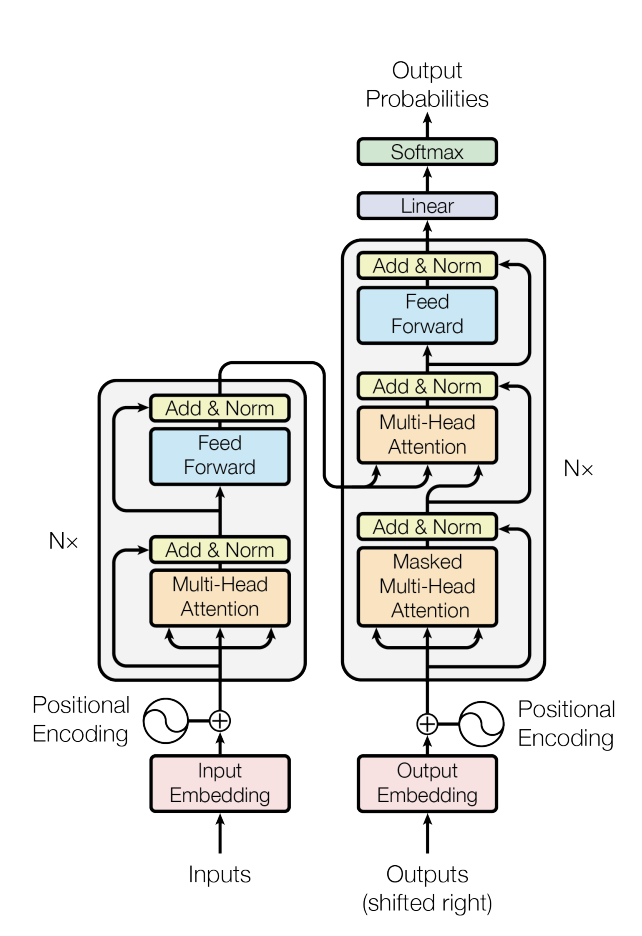
\includegraphics[width=0.5\textwidth, scale=0.8]{figures/2-sota/transformer.png}
    \caption[Transformer]{\textbf{Transformer} --- This illustration was taken from \cite{vaswani_attention_2017} and shows the general architecture of the base transformer. One can see that the constituents are pretty simple. These are simple word embeddings (which are not covered in this study), self-attention, and feedforward layers. The left side of the structure is called the encoder, while the right side is called the decoder.}
    \label{fig:transformer}
\end{figure}
\paragraph{Vector Quantised Variational AutoEncoder (VQ-VAE) (2018)} \label{sec:vq-vae}

The \acf{VQ-VAE}, introduced in 2018, model distinguishes itself from traditional \acp{VAE} in two main aspects: the encoder network outputs discrete codes instead of continuous ones, and the prior is learned rather than static. While continuous feature learning has been the focus of many previous works, this model, introduced by \cite{oord_neural_2018}, concentrates on discrete representations, a natural fit for complex reasoning, planning, and predictive learning.

The \ac{VQ-VAE} model combines the \ac{VAE} framework with discrete latent representations through a parameterization of the posterior distribution of (discrete) latents given an observation. Based on vector quantization, this model is simple to train, does not suffer from significant variance, and avoids the ``posterior collapse''. As illustrated in Fig~\ref{fig:vq-vae}, the \ac{VQ-VAE} architecture consists of an encoder, a discrete latent space, and a decoder.

\begin{figure*}[ht]
    \centering
    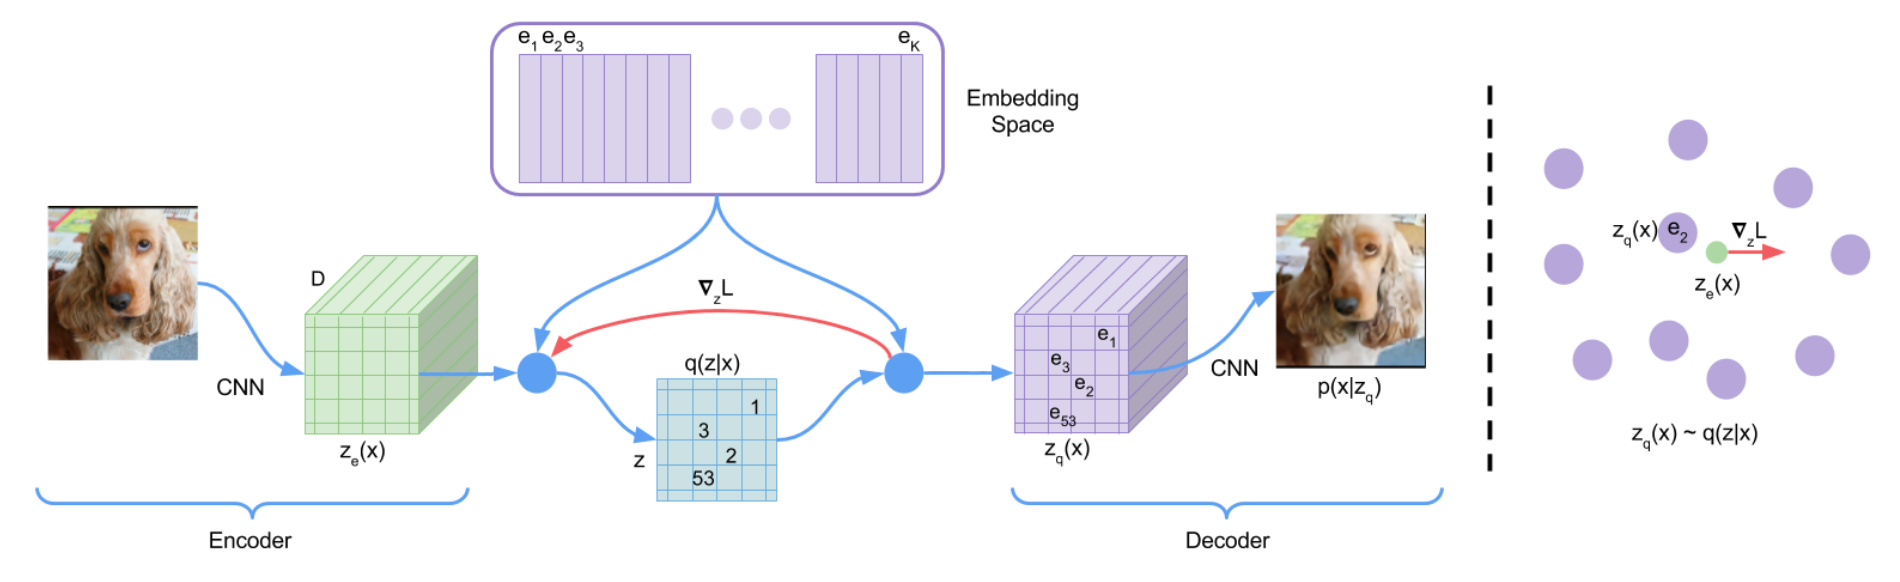
\includegraphics[width=\textwidth]{figures/2-sota/vq-vae.png}
    \caption[VQ-VAE]{\textbf{VQ-VAE} --- Taken from the original paper, this Figure presents two distinct illustrations. On the left side, a detailed diagram of the \ac{VQ-VAE} architecture is provided, showcasing the flow of information through the encoder, the discrete latent space, and the decoder. On the right side, a visualization of the embedding space is displayed, where the encoder output $z(X)$ is mapped to its nearest embedding point $e_2$. The red arrow represents the gradient $\nabla_z L$, influencing the encoder's output adjustment. This adjustment may result in a different configuration during the subsequent forward pass, highlighting the dynamic nature of the learning process within the \ac{VQ-VAE} model.}
    \label{fig:vq-vae}
\end{figure*}

The \ac{VQ-VAE} defines a latent embedding space $e \in R^{N \times D}$, where $N$ is the size of the discrete latent space (i.e., a $N$-way categorical), and $D$ is the dimensionality of each latent embedding vector $e_n$. There are $N$ embedding vectors $e_n \in R^D, n \in 1, 2, ..., N$. The model takes an input $X$, passed through an encoder producing output $z_e(X)$. The discrete latent variables $z$ are then calculated by the nearest neighbor look-up using the shared embedding space $e$. The input to the decoder is the corresponding embedding vector $e_n$. This forward computation pipeline is a regular autoencoder with a non-linearity that maps the latents to 1-of-N embedding vectors.

The posterior categorical distribution $q(z|X)$ probabilities are defined as one-hot (Eq. \ref{eq:vq-vae-posterior}):

\begin{equation} \label{eq:vq-vae-posterior}
  q(z = n|X) =
  \begin{cases}
    1 & \text{for } n = \text{argmin}_j ||z_e(X)-e_j||_2, \\
    0 & \text{otherwise}.
  \end{cases}
\end{equation}

where $z = e_n$ is the closest embedding vector to the encoder output $z_e(X)$. During forward computation, the nearest embedding $z_q(X)$ is passed to the decoder, and during the backward pass, the gradient $\nabla_z L$ is passed unaltered to the encoder. The overall loss function has three components to train different parts of the \ac{VQ-VAE}: the reconstruction loss, the \ac{VQ} objective, and the commitment loss. The total training objective becomes:

\setlength{\arraycolsep}{0.0em}
\begin{eqnarray}
\label{eq:vq-vae-loss}
\label{eq:reconstruction-loss}L&{}={}&\log p(X|z_q(X))\\
\label{eq:vq-objective}&&{+}\:||\text{sg}[z_e(X)] - e||_2^2\\
\label{eq:commitment-loss}&&{+}\:\beta||z_e(X) - \text{sg}[e]||_2^2
\end{eqnarray}
\setlength{\arraycolsep}{5pt}

This equation combines the three following terms:
\begin{enumerate}
	\item \textbf{Reconstruction loss} (Equation \ref{eq:reconstruction-loss}): This term represents the log probability of the input data $X$ given the latent variable  $z_q(X)$. It measures how well the model can reconstruct the input data using $z_q(X)$ as a representation. Maximizing this term would lead to a better reconstruction of the input data.
	\item \textbf{\Ac{VQ}} (Equation \ref{eq:vq-objective}): The second term measures the difference between the stop-gradient of the encoder output $z_e(X)$ and the embedding vector $e$. The stop-gradient operator, denoted as $\text{sg}$, acts as the identity during the forward pass but has zero partial derivatives during the backward pass. This term encourages the model to use the embeddings effectively by minimizing the distance between the encoder output and the closest embedding vector.
	\item \textbf{Commitment loss} (Equation \ref{eq:commitment-loss}): This term acts as a regularization term that measures the difference between the encoder output $z_e(X)$ and the stop-gradient of the embedding vector $e$. The  $\beta$ parameter controls the strength of this regularization. Minimizing this term would make $z_e(X)$  closer to the straight-through estimator of $e$.
\end{enumerate}

VQ-VAE has emerged as a vital component in generative artificial intelligence, spanning domains such as image~\cite{ramesh_zero-shot_2021} and sound generation~\cite{yang_diffsound_2022}.
\paragraph{Multi-Scale Vector Quantised Variational AutoEncoder (MS-VQ-VAE) (2019)} \label{sec:ms-vq-vae}

The \acf{MS-VQ-VAE} model is a generalization of the \ac{VQ-VAE} model (see Section \ref{sec:vq-vae}) that employs multiple discrete latent spaces with different scales and dimensions. Tjandra et al. proposed this model \cite{tjandra_vqvae_2019} to learn unsupervised hierarchical and discrete representations of complex data. The \ac{MS-VQ-VAE} architecture comprises an encoder, a multiscale discrete latent space, and a decoder.

The key difference between the \ac{MS-VQ-VAE} and the \ac{VQ-VAE} is that the former defines a collection of latent embedding spaces $e^s \in R^{K_s \times D_s}$, where $s$ denotes the scale index, $K_s$ denotes the cardinality of the discrete latent space at scale $s$, and $D_s$ denotes the dimensionality of each latent embedding vector $e^s_i$. There are $K_s$ embedding vectors $e^s_i \in R^{D_s}, i \in 1, 2, ..., K_s$. The model takes an input $x$, encoded into outputs $z_e^s(x)$ at different scales. The discrete latent variables $z^s$ are then obtained by the nearest neighbor look-up using the shared embedding space $e^s$. The decoder input is the corresponding embedding vector $e^s_k$. This forward computation pipeline resembles a regular \ac{AE} (see section \ref{sec:autoencoders}) with a non-linearity that maps the latents to 1-of-$K_s$ embedding vectors.

The posterior categorical distribution $q(z^s|x)$ probabilities are defined as one-hot (Eq. \ref{eq:ms-vq-vae-posterior}), analogous to Eq. \ref{eq:vq-vae-posterior} in section \ref{sec:vq-vae}, but with an additional scale index:

\begin{equation} \label{eq:ms-vq-vae-posterior}
 q(z^s = k|x) = \begin{cases}
 1 & \text{for } k = \text{argmin}_j ||z_e^s(x)-e^s_j||_2, \\
 0 & \text{otherwise}.
 \end{cases}
\end{equation}

The overall loss function consists of three components for each scale: the reconstruction loss, the VQ objective, and the commitment loss. The total training objective becomes (Eq. \ref{eq:ms-vq-vae-loss}), analogous to Eq. \ref{eq:vq-vae-loss} in section \ref{sec:vq-vae}, but with a summation over scales:

\begin{equation} \label{eq:ms-vq-vae-loss}
 L = \sum_{s=1}^{S} (\log p(x|z_q^s(x)) + ||\text{sg}[z_e^s(x)] - e^s||_2^2 + \beta||z_e^s(x) - \text{sg}[e^s]||_2^2)
\end{equation}

The benefit of using multiple codebooks and scales is that it enables the model to capture different levels of abstraction and granularity in audio signals. For instance, lower scales can encode phonetic information in speech, while higher scales can encode prosodic information. Furthermore, using multiple codebooks can enhance the diversity and expressiveness of the latent space by allowing more combinations of discrete codes.